\documentclass[12pt]{article}

%%%%%%%%%%%%%%%%%%%%%%%%%%%%%%%%%%%%%%%%%%%%%%%%%%%%%%%%%%%%%%%%%%%
%%%%% Page Margins
\usepackage[letterpaper,portrait,margin=1in]{geometry}
%%%%%%%%%%%%%%%%%%%%%%%%%%%%%%%%%%%%%%%%%%%%%%%%%%%%%%%%%%%%%%%%%%%

%%%% Packages
%%%%%%%%%%%%%%%%%%%%%%%%%%%%%%%%%%%%%%%%%%%%%%%%%%%%%%%%%%%%%%%%%%%
\usepackage{amssymb}
\usepackage{graphicx}
\usepackage{amsmath,amsfonts,amsthm}
\usepackage{enumerate}
\usepackage{setspace}
  \onehalfspacing
\usepackage{mathtools}
\usepackage{booktabs,array}
\usepackage{natbib}
\newcommand{\citeasnoun}[1]{\citet{#1}}
\usepackage{caption}
\captionsetup{margin=\parindent,indention=\parindent,font=small,labelfont=sc}

\usepackage[svgnames]{xcolor}
\definecolor{blue1}{RGB}{25,25,112}
\definecolor{ink}{RGB}{30,30,35}
\definecolor{muted}{RGB}{120,125,135}
\definecolor{accent}{RGB}{185,80,30}
\definecolor{poscol}{RGB}{35,110,70}
\definecolor{negcol}{RGB}{165,45,45}

\usepackage{tikz}
\usetikzlibrary{arrows.meta,decorations.pathreplacing}

\usepackage{hyperref}
\hypersetup{bookmarksnumbered=true,
            colorlinks=true,
            citecolor=blue1,urlcolor=blue1,linkcolor=blue1,
          }
\allowdisplaybreaks

%%%%%%%%%%%%%%%%%%%%%%%%%%%%%%%%%%%%%%%%%%%%%%%%%%%%%%%%%%%%%%%%%%%%%%%%%%%
%%%% Theorems & Proofs
%%%%%%%%%%%%%%%%%%%%%%%%%%%%%%%%%%%%%%%%%%%%%%%%%%%%%%%%%%%%%%%%%%%%%%%%%%%
\newtheoremstyle{mystyle}% name
  {}{}{\itshape}{}{\scshape}{.}{ }{}

\theoremstyle{mystyle}
\newtheorem{definition}{Definition}
\newtheorem{corollary}{Corollary}
\newtheorem{theorem}{Theorem}
\newtheorem{lemma}{Lemma}
\newtheorem{proposition}{Proposition}

\newtheoremstyle{mystyle2}% name
  {}{}{\upshape}{}{\scshape}{.}{ }{}

\theoremstyle{mystyle2}
\newtheorem{example}{Example}
\newtheorem{assumption}{Assumption}
\newtheorem{remark}{Remark}

\renewcommand{\proofname}{\upshape\scshape Proof}
\newenvironment{sketch}{\begin{quote}\small\noindent\textit{Proof sketch.}}{\end{quote}}

%%%%%%%%%%%%%%%%%%%%%%%%%%%%%%%%%%%%%%%%%%%%%%%%%%%%%%%%%%%%%%%%%%%%%%%%%%%%%
%%%% Title Page
%%%%%%%%%%%%%%%%%%%%%%%%%%%%%%%%%%%%%%%%%%%%%%%%%%%%%%%%%%%%%%%%%%%%%%%%%%%
\renewcommand{\abstractname}{{\normalfont\textsc{Abstract}}}

\newenvironment{keywords}%
       {\list{\textsc{Keywords:}}%
              {\setlength{\listparindent}{\parindent}
               \setlength{\parsep}{\parskip}
               \setlength{\leftmargin}{0in}
               \setlength{\rightmargin}{0in}
               \setlength{\itemindent}{-\leftmargin}
                  \addtolength{\itemindent}{\labelwidth}
                  \addtolength{\itemindent}{\labelsep}
               }
        \item}
       {\endlist\par}
\newenvironment{JEL}%
       {\list{\textsc{JEL Classification Numbers:}}%
              {\setlength{\listparindent}{\parindent}
               \setlength{\parsep}{\parskip}
               \setlength{\leftmargin}{0in}
               \setlength{\rightmargin}{0in}
               \setlength{\itemindent}{-\leftmargin}
                  \addtolength{\itemindent}{\labelwidth}
                  \addtolength{\itemindent}{\labelsep}
               }
        \item}
       {\endlist\par}

%%%%%%%%%%%%%%%%%%%%%%%%%%%%%%%%%%%%%%%%%%%%%%%%%%%%%%%%%%%%%%%%%%%%%%%%%%%%%%%
%%%% Sections and Subsections
%%%%%%%%%%%%%%%%%%%%%%%%%%%%%%%%%%%%%%%%%%%%%%%%%%%%%%%%%%%%%%%%%%%%%%%%%%%
\makeatletter
\newcommand{\mmpfont}{\scshape}
\renewcommand\section{\@startsection {section}{1}{\z@}%
                                   {-3.5ex \@plus -1ex \@minus -.2ex}%
                                   {2.3ex \@plus .2ex}%
                                   {\normalfont\large\mmpfont}}
\renewcommand\subsection{\@startsection{subsection}{2}{\z@}%
                                     {-3.25ex\@plus -1ex \@minus -.2ex}%
                                     {1.5ex \@plus .2ex}%
                                     {\normalfont\normalsize\mmpfont}}
\renewcommand\subsubsection{\@startsection{subsubsection}{3}{\z@}%
                                    {-2.5ex\@plus -1ex \@minus -.2ex}%
                                     {1.5ex \@plus .2ex}%
                                     {\normalfont\normalsize\mmpfont}}
\renewcommand\paragraph{\@startsection{paragraph}{4}{\z@}%
                                    {2.5ex \@plus 1ex \@minus -.2ex}%
                                    {-1em}%
                                    {\normalfont\normalsize\mmpfont}}
\makeatother

%%%%%%%%%%%%%%%%%%%%%%%%%%%%%%%%%%%%%%%%%%%%%%%%%%%%%%%%%%%%%%%%%%%%%%%%%%%%%
%%%%% Document-specific macros %%%%%%%%%%%%%%%%%%%%%%%%%%%%%%%%%%%%%%%%%%%%%%
%%%%%%%%%%%%%%%%%%%%%%%%%%%%%%%%%%%%%%%%%%%%%%%%%%%%%%%%%%%%%%%%%%%%%%%%%%%%%
\newcommand{\EV}[1]{\mathbb{E}[#1]}
\newcommand{\M}{\mathcal{M}}
\newcommand{\cP}{\mathcal{P}}
\newcommand{\bmm}{\mathbf{m}}
\newcommand{\SPA}{\mathrm{SPA}}
\newcommand{\1}{\mathbf{1}}
\renewcommand{\Re}{\mathbb{R}}

\newcommand{\qpathpanel}[3]{%
\begin{tikzpicture}[scale=2.0]
  \draw[-{Stealth[length=1.6mm]},muted,line width=0.5pt] (0,0)--(1.12,0) node[below,font=\scriptsize,text=muted]{$q$};
  \draw[-{Stealth[length=1.6mm]},muted,line width=0.5pt] (0,0)--(0,1.12) node[left,font=\scriptsize,text=muted]{$t$};
  \draw[muted,dashed,line width=0.5pt] (0,0)--(1,1);
  #2
  \node[font=\footnotesize\scshape,anchor=south] at (0.55,1.14) {#1};
  \node[font=\scriptsize,text=muted,anchor=north] at (0.55,-0.12) {#3};
\end{tikzpicture}}

\title{
\textsc{Auction Design under Competition}\thanks{I thank seminar audiences at Arizona State, UC Berkeley, UCLA, Yale, Google Research, and the INFORMS Annual Meeting for helpful comments. This paper supersedes an earlier working paper circulated under the title ``Competing Auctioneers.''}
}

\author{
   \textsc{Mallesh M. Pai}\thanks{Department of Economics, Rice University.
   Email: \href{mailto:mallesh.pai@rice.edu}{mallesh.pai@rice.edu}.}
}

\date{\normalsize \textsc{November 2026}}

\hypersetup{hypertexnames=false}
\begin{document}
\maketitle

\begin{abstract}
A monopolist designing an optimal auction may withhold the good (via a reserve) or misallocate it (by pooling types and rationing randomly). Both distortions vanish under perfect competition, whereas existing oligopoly models restrict sellers to second price auctions and assume misallocation away. We let $m$ sellers compete for $n$ buyers via auctions with a reserve and finitely many pooling intervals, and express a seller's revenue in terms of Cournot oligopoly revenues---so Cournot's marginal revenue $\psi_m(v)=v-\frac{1}{m}\frac{1-F(v)}{f(v)}$ replaces Myerson's virtual valuation. When all buyer values lie strictly above cost, monotone nonnegative $\psi_m$ ensures symmetric second price auctions survive all deviations for every~$n$, and monotonicity is tight across~$n$. When reserves bind, symmetric second price auctions never survive---an asking price captures marginal buyers---and asymmetric duopoly profiles with negative virtual valuation at the higher reserve also fail for large~$n$.
\end{abstract}

{\small
\begin{keywords}
optimal auctions, competition, misallocation, directed search, majorization
\end{keywords}
\begin{JEL}
C72, D44, D82
\end{JEL}
}

\newpage

%%%%%%%%%%%%%%%%%%%%%%%%%%%%%%%%%%%%%%%%%%%%%%%%%%%%%%%%%%%%%%%%%%%%
\section{Introduction}
%%%%%%%%%%%%%%%%%%%%%%%%%%%%%%%%%%%%%%%%%%%%%%%%%%%%%%%%%%%%%%%%%%%%

Optimal auction design for a single seller is well understood. As \citeasnoun{bulow1989} emphasize, the virtual valuation $\psi_1(v)=v-\frac{1-F(v)}{f(v)}$ of \citeasnoun{myerson} is the marginal revenue of a monopolist facing demand curve $1-F$. Seen through this lens, a revenue-maximizing monopolist may introduce two distinct inefficiencies. First, he \emph{withholds} the good from buyers whose virtual valuation is negative by setting a reserve price above cost. Second, when $\psi_1$ is not nondecreasing---failing Myerson's \emph{regularity} condition---he \emph{misallocates} the good: he irons the virtual valuation by pooling an interval of buyer types and allocating randomly among them, so a lower-value buyer can win even when a higher-value buyer is present. A posted price with random rationing is the extreme instance of misallocation. A second price auction with a reserve, by contrast, may withhold the good but never misallocates it.

At the opposite extreme of perfect competition, \citeasnoun{mcafee}, \citeasnoun{peters1997}, and \citeasnoun{peters} show that in a large market both inefficiencies disappear: every seller offering a second price auction with reserve equal to cost is an equilibrium, regardless of the distribution of buyer values. What happens in between, under finite oligopoly? The literature following \citeasnoun{burguet} and \citeasnoun{virag2010competing} restricts competing sellers to second price auctions with reserves. That restriction lets us study how competition disciplines withholding, while ruling out misallocation by assumption. In doing so, it takes for granted that the mechanism format optimal under monopoly (when $F$ is regular) and under perfect competition remains optimal under oligopoly.

This paper drops that restriction and asks when misallocation arises among competing sellers. We study a market with $m\ge 2$ sellers, each holding one unit of an identical good with zero cost, and $n\ge 2$ buyers whose private valuations are i.i.d.\ draws from a distribution $F$ on $[a,1]$. Sellers simultaneously announce \emph{hierarchical mechanisms}: a reserve price together with a (possibly empty) finite collection of disjoint pooling intervals on which bids are treated identically and ties are broken uniformly at random, with Vickrey payments pinned down by incentive compatibility. This class includes second price auctions, posted prices, asking prices, and Myerson's ironed auctions, and is motivated by the extreme points of the Border-feasible set of interim allocation rules \citep{kleiner2021}. After observing the announcements, each buyer privately learns her valuation and chooses one seller to visit; each seller then runs his announced mechanism among his visitors.

The technical obstacle in finite competing-mechanism games is well known: a seller's choice of mechanism determines both which buyers visit him and what surplus those buyers earn elsewhere. Both the distribution of visitors and buyers' type-dependent outside options are endogenous, so standard screening techniques \citep{jullien,rochet} do not apply. We overcome this in two steps. First, although pooling breaks the welfare-potential structure of the visit stage under second price auctions, we show that after any unilateral deviation by a single seller the sequentially rational continuation of the visit game exists, is unique in effective distributions, and takes a simple localized form (Proposition~\ref{prop:unique}). Second, we represent any continuation by the deviator's \emph{quantity path}: the mass $t(q)$ of buyers above a type who visit the deviator as a function of the mass $q$ visiting each rival. In these coordinates, a seller's revenue equals a weighted integral of Cournot oligopoly revenues $\Pi(t,q)=t\,P(t+(m-1)q)$ (with inverse demand $P(z)=F^{-1}(1-z)$), plus a baseline reserve term and less any extra rent left to strictly preferring buyers, while Border's feasibility constraint yields a family of integral bounds saying that a seller cannot allocate more than his rivals to the top of the market (Proposition~\ref{prop:path}).

This Cournot representation organizes our main results into four findings, splitting sharply by whether the market is \emph{covered} ($a>0$, so every buyer values the good strictly above cost) or reserves \emph{bind} (sitting at or above $a$).

First, away from the bottom of the market, Cournot's marginal revenue
\[
\psi_m(v) = v - \frac{1}{m}\,\frac{1-F(v)}{f(v)}
\]
replaces Myerson's virtual valuation. If $\psi_m$ is nondecreasing, no seller gains by adding any finite collection of pooling intervals whose effect stays in the interior of the market, for any number of buyers (Theorem~\ref{thm:cournot}). Competition scales the monopolist's markup term by the Cournot conduct parameter $1/m$, interpolating smoothly from Myerson ($m=1$) to McAfee ($m\to\infty$). Equivalently, writing $\psi_m(v)=\bigl(1-\frac{1}{m}\bigr)v+\frac{1}{m}\psi_1(v)$, an oligopolist evaluates interior misallocation as if he were a monopolist placing welfare weight $1-\frac{1}{m}$ on buyer surplus.

Second, in a covered market ($a>0$), \citeasnoun{virag2010competing} identified a unique symmetric candidate with a non-binding reserve among second price auctions: a reserve $\rho^*=\frac{(n-1)a}{(m-1)^2+n-1}<a$ that excludes no buyer. We show that if $\psi_m$ is nondecreasing on $[a,1]$ and $\psi_m(a)\ge 0$, then all sellers posting second price auctions with reserve $\rho^*$ is an equilibrium against all hierarchical deviations, for every $n\ge 2$ and $m\ge 2$ (Theorem~\ref{thm:covered}). Monotonicity and nonnegativity of $\psi_m$ also rule out all reserve deviations globally, so no separate assumption on the reserve-only game is needed. In particular, second price auctions can form an equilibrium even when $F$ fails Myerson's regularity and a monopolist would iron (Example~\ref{ex:pareto}).

Third, when reserves bind ($\rho\ge a$), competition creates a new reason to misallocate that has no monopoly counterpart. At any symmetric profile of second price auctions with a positive binding reserve $\rho\in(0,1)$, a seller strictly raises revenue by pooling an interval of buyers just above $\rho$---an \emph{asking price}---for every distribution $F$, every $m\ge 2$, and every $n\ge 2$; when $a=0$, no symmetric profile of second price auctions is an equilibrium (Theorem~\ref{thm:bind}). Because buyers just above $\rho$ earn virtually zero surplus at rivals, an asking price captures a net gain in traffic at price $\rho$ while equalizing winning probabilities across the captured segment so that capture does not unravel from below. Asymmetric duopoly profiles fare no better for large~$n$: when $a=0$, along any sequence of asymmetric second price auctions whose reserves converge to distinct limits $r_L<r_H<1$ with $\psi_1(r_H)<0$, the low-reserve seller strictly profits for all sufficiently large~$n$ by raising his reserve and adding a pool straddling the cutoff type where buyers split between sellers (Theorem~\ref{thm:asym}).

Fourth, we analyze how sharp Cournot's condition is (Section~\ref{sec:sharp} and Appendix~\ref{app:sharp}). When $f$ is differentiable, monotonicity of $\psi_m$ is equivalent to an upper bound on the curvature of demand (formally defined in Section~\ref{sec:sharp}) that tightens from $2$ under monopoly to $m+1$ under $m$-seller oligopoly. For narrow pools at any fixed $n\ge 2$, re-sorting across sellers disciplines a deviator slightly more than Cournot's $1/m$, replacing $1/m$ with a strictly smaller weight $\varpi(m)=\frac{m+1}{m^2+2m-1}$. As $n$ grows large, however, wide pools reaching toward the top of the market become the binding deviation, and Cournot's curvature bound $m+1$ cannot be improved uniformly across~$n$ (Theorem~\ref{thm:sharp}).

The remainder of the paper is organized as follows. Section~\ref{sec:model} sets out the model. Section~\ref{sec:visits} characterizes the visit stage and establishes uniqueness after any unilateral deviation. Section~\ref{sec:cournot} develops the quantity-path representation and states the covered-market equilibrium theorem. Section~\ref{sec:binding} turns to binding reserves and establishes the failure of symmetric profiles and asymmetric large-$n$ duopoly profiles. Section~\ref{sec:sharp} summarizes the sharpness of Cournot's condition. Section~\ref{sec:rellit} discusses related literature, and Section~\ref{sec:conclude} concludes with open questions. All proofs appear in Appendices~\ref{app:visits}--\ref{app:sharp}.

%%%%%%%%%%%%%%%%%%%%%%%%%%%%%%%%%%%%%%%%%%%%%%%%%%%%%%%%%%%%%%%%%%%%
\section{Model} \label{sec:model}
%%%%%%%%%%%%%%%%%%%%%%%%%%%%%%%%%%%%%%%%%%%%%%%%%%%%%%%%%%%%%%%%%%%%

\subsection{The Market}
There are $m\ge 2$ risk-neutral sellers, indexed by $j\in\{1,\dots,m\}$, each endowed with one unit of an identical indivisible good valued at zero. There are $n\ge 2$ risk-neutral buyers with unit demand. Buyer $i$'s private valuation $v_i$ is drawn independently from a common distribution $F$ with density $f$ on $[a,1]$, where $0\le a<1$; we extend $F\equiv 0$ and $f\equiv 0$ on $[0,a)$. Since sellers' cost is normalized to zero, $a$ represents the smallest possible gain from trade. We call the market \emph{covered} if $a>0$, so that every buyer values the good strictly above cost, and we call a reserve price $\rho$ \emph{slack} if $\rho<a$ and \emph{binding} if $\rho\ge a$.

\begin{assumption}\label{a:one}
The density $f$ is continuous on $[a,1]$ with $\underline f:=\min_{v\in[a,1]} f(v)>0$.
\end{assumption}

\begin{assumption}\label{a:two}
$f\in C^1([a,1])$, and we write $K:=\max_{v\in[a,1]} |f'(v)|$.
\end{assumption}

\emph{Standing convention.} Throughout the paper, $m,n\ge 2$ and Assumption~\ref{a:one} are maintained without repeated mention. Assumption~\ref{a:two} is stated explicitly wherever it is invoked (Section~\ref{sec:sharp} and Appendix~\ref{app:sharp}).

The game $\Gamma$ unfolds in three stages:
\begin{enumerate}
\item Sellers simultaneously announce mechanisms from the class defined in Section~\ref{sec:pss}.
\item Buyers observe all announcements, privately learn their own valuations $v_i$, and simultaneously choose one seller to visit.\footnote{Allowing buyers to abstain is equivalent to visiting a seller whose reserve excludes them (or, when all reserves are zero, yields zero surplus, which is weakly dominated by visiting any seller), so restricting buyers to choose one seller is without loss.}
\item Each seller executes his announced mechanism among the buyers who visit him.
\end{enumerate}

We restrict attention to anonymous mechanisms (outcomes depend only on reports, not buyer identities) and buyer-symmetric visit strategies (a buyer's visit probabilities depend only on her valuation, not her identity).

\subsection{Hierarchical Mechanisms} \label{sec:pss}

Because the number and valuation distribution of a seller's visitors are determined endogenously in Stage~2, a seller cannot announce a mechanism via its interim allocation rule. Instead, a seller specifies an ex-post allocation rule through two primitives: a reserve price below which he refuses to sell, and a collection of report intervals that he treats as identical.

\begin{definition}[\textsc{Hierarchical Mechanisms}]\label{def:purestrat}
A \emph{hierarchical mechanism} is a pair $\bmm=(r,\cP)$ consisting of a reserve price $r\in[0,1]$ and a finite collection $\cP$ of pairwise disjoint open \emph{pooling intervals} in $(r,1)$. Buyers with reports below $r$ are ineligible. Eligible buyers are ranked by their reports, except that reports lying in a common interval $I\in\cP$ are ranked as tied. Ties are broken using a uniform random priority order over eligible buyers drawn independently of reports; the good is awarded to the highest-ranked eligible buyer (using the priority order within a tied group), and conditional on the priority draw the winner pays the lowest report at which she would still have won (Vickrey pricing). We denote the class of hierarchical mechanisms by $\M$, write $\SPA(r):=(r,\emptyset)$ for a \emph{standard (second price) auction} with reserve $r$, and write $\SPA(\rho)^m$ for the symmetric profile in which every seller posts $\SPA(\rho)$. We refer to the restricted game in which sellers choose only standard auctions $\SPA(r)$ as the \emph{reserve game}.
\end{definition}

Conditional on any realization of the priority draw, the allocation rule is monotone in a visitor's report, so bidding one's true valuation is weakly dominant for every visitor regardless of who else visits the seller; we select truthful bidding at Stage~3. Definition~\ref{def:purestrat} encompasses the formats used across the auction and directed-search literatures:
\begin{itemize}
\item $\SPA(r)=(r,\emptyset)$ is a standard second price auction, which may withhold the good ($r>a$) but never misallocates it among visitors;
\item $(p,\{(p,1)\})$ is a posted price $p$ with uniform random rationing;
\item $(r,\{(r,\beta)\})$ is an \emph{asking price} (buyers can purchase at $r$, subject to rationing, or bid above $\beta$ to preempt);
\item $(r,\{(\alpha_1,\beta_1),\dots,(\alpha_k,\beta_k)\})$ is a general Myerson-style ironed auction.
\end{itemize}

This class excludes mechanisms that condition on the realized number of visitors or randomize ex post after visits are made (such as random reserves). Nevertheless, hierarchical mechanisms have a natural reduced-form motivation. Given $n$ buyers drawing i.i.d.\ values from any effective distribution $G$, \citeasnoun{border1} shows that a nondecreasing interim winning-probability rule $x$ is implementable if and only if
\begin{equation}\label{eq:border}
n\int_v^1 x(u)\,dG(u)\ \le\ 1 - G(v)^n \qquad \text{for all } v.
\end{equation}
In quantile space, \eqref{eq:border} states that $x$ is weakly majorized by the assortative rule $y\mapsto y^{n-1}$ of the efficient auction. As \citeasnoun{kleiner2021} show, the extreme points of this majorization polytope are the rules that are zero below a cutoff, efficient on some intervals, and constant on countably many pooling intervals.\footnote{See \citeasnoun{che2013} for Border's characterization with atoms (such as the atom at zero induced by buyers who visit other sellers), \citeasnoun{hartreny2015} for direct implementation, and Theorem~1 of \citeasnoun{kleiner2021} for the extreme-point characterization. Definition~\ref{def:purestrat} restricts to finitely many pooling intervals; because visits are endogenous, this class is a structural choice rather than a without-loss reduction.} Definition~\ref{def:purestrat} therefore specifies the finitely ironed extreme points ex post, without reference to the endogenous visitor distribution.

\subsection{The Visit Stage and Solution Concept}

Let $\Delta^m:=\{p\in\Re_+^m:\sum_{j=1}^m p_j=1\}$. After observing a mechanism profile $(\bmm_1,\dots,\bmm_m)\in\M^m$, buyers play a visit subgame. A symmetric visit strategy is a measurable map $\theta:[a,1]\to\Delta^m$, where $\theta_j(v)$ is the probability that a buyer of valuation $v$ visits seller $j$.

To avoid working with multinomial distributions over visitor counts, we treat any buyer who visits another seller as submitting an ineligible phantom bid of $0$ at seller $j$ (which never wins, even when $r_j=0$). Seller $j$ then faces $n$ i.i.d.\ effective bids drawn from the \emph{effective distribution}
\[
F_j(v) = 1 - \int_v^1 \theta_j(u)f(u)\,du,
\]
which carries an atom of size $F_j(a)=1-\int_a^1\theta_j(u)f(u)\,du$ at zero (the probability a buyer visits elsewhere). Under $\bmm_j=(r_j,\cP_j)$, a visitor of type $v$ faces $n-1$ independent draws from $F_j$, so her interim winning probability is $x_j(v)=0$ for $v<r_j$, $x_j(v)=F_j(v)^{n-1}$ for $v\ge r_j$ outside $\bigcup\cP_j$, and on each pooling interval $(\alpha,\beta)\in\cP_j$,
\begin{equation}\label{eq:poolalloc}
x_j(v) = \bar x_j(\alpha,\beta) := \begin{cases}
\dfrac{F_j(\beta)^n - F_j(\alpha)^n}{n\bigl(F_j(\beta)-F_j(\alpha)\bigr)} & \text{if } F_j(\beta)>F_j(\alpha),\\[6pt]
F_j(\alpha)^{n-1} & \text{if } F_j(\beta)=F_j(\alpha).
\end{cases}
\end{equation}
Under the priority-order Vickrey rule of Definition~\ref{def:purestrat}, averaging payments over the independent priority draw yields the standard envelope formulas for a type-$v$ visitor's interim surplus, expected payment at seller $j$, and seller $j$'s expected revenue:
\begin{equation}\label{eq:payoffs}
s_j(v) = \int_0^v x_j(u)\,du, \qquad p_j(v) = v\,x_j(v) - s_j(v), \qquad R_j = n\int_a^1 p_j(v)\,\theta_j(v)f(v)\,dv.
\end{equation}

A visit strategy $\theta$ is \emph{sequentially rational} (SR) if, for almost every $v\in[a,1]$, $\theta_j(v)>0$ implies $s_j(v)=\max_k s_k(v)$. Our solution concept for $\Gamma$ is weak perfect Bayesian equilibrium in buyer-symmetric strategies: visit strategies must be sequentially rational after every mechanism profile, and no seller can strictly increase expected revenue by a unilateral deviation in $\M$, anticipating the resulting continuation play. As we show next, an SR continuation exists after every profile in $\M^m$, and after any unilateral deviation from $\SPA(\rho)^m$ it is unique in effective distributions, so equilibrium payoffs are completely independent of any selection rule.

%%%%%%%%%%%%%%%%%%%%%%%%%%%%%%%%%%%%%%%%%%%%%%%%%%%%%%%%%%%%%%%%%%%%
\section{The Visit Stage} \label{sec:visits}
%%%%%%%%%%%%%%%%%%%%%%%%%%%%%%%%%%%%%%%%%%%%%%%%%%%%%%%%%%%%%%%%%%%%

We begin by solving the buyer visit subgame, first when all sellers announce standard auctions and then after an arbitrary unilateral deviation to a hierarchical mechanism. Throughout the paper, let
\[
A(v) := 1 - \frac{1-F(v)}{m}
\]
denote the symmetric effective distribution induced when buyers split uniformly across all $m$ sellers. All proofs for this section appear in Appendix~\ref{app:visits}.

\subsection{Standard Auctions: A Potential Game}

When every seller runs a second price auction, a visitor's realized surplus equals her marginal contribution to reserve-truncated welfare at the seller she visits. Consequently, the visit subgame is an exact potential game \citep{monderer1996} whose potential is expected truncated welfare summed across sellers.

\begin{proposition}[\textsc{Standard Auctions}]\label{prop:pot}
Suppose every seller $j$ posts $\SPA(r_j)$. Then an SR visit strategy exists; $\theta$ is SR if and only if it maximizes the concave potential
\begin{equation}\label{eq:pot}
\Phi(\theta) = \sum_{j=1}^m \int_{r_j}^1 \bigl[1 - F_j(v)^n\bigr]\,dv;
\end{equation}
and all SR strategies induce the same effective distributions on $(r_j,1]$, hence the same allocations, buyer surpluses, and seller revenues. In particular:
\begin{enumerate}[(i)]
\item If every seller posts $\SPA(\rho)$, the uniform split $\theta_j\equiv\frac{1}{m}$ is SR, and every SR continuation induces $F_j=A$ on $[\rho,1]$.
\item If seller $1$ posts $\SPA(r_1)$ with $r_1>\rho$ while all rivals post $\SPA(\rho)$, there is a unique cutoff $w\in[\max\{r_1,a\},1]$ such that buyers in $(\max\{\rho,a\},w)$ visit rivals with symmetric effective distributions and buyers above $w$ split uniformly across all $m$ sellers. Symmetrically, if $r_1<\rho$, there is a unique cutoff $w\in[\max\{\rho,a\},1]$ such that buyers in $(\max\{r_1,a\},w)$ visit seller $1$ exclusively and buyers above $w$ split uniformly. In both cases, $w$ varies continuously and monotonically with $r_1$.
\end{enumerate}
\end{proposition}

Part~(ii) recovers the single-deviator cutoff of \citeasnoun{burguet} (explicitly characterized in \eqref{eq:w} and \eqref{eq:w_rev} in Appendix~\ref{app:visits}). The logic is straightforward: a buyer with value just above $r_1>\rho$ earns nearly zero surplus at seller $1$ and therefore strictly prefers a rival. Only types above the indifference cutoff $w$ visit seller $1$, and because all sellers are efficient above $w$, indifference forces equal effective distributions $F_j=A$ there.

\subsection{Uniqueness after Any Unilateral Deviation}

When a seller introduces a pooling interval, a pooled buyer's winning probability depends on the mass of buyers \emph{below} her inside the pool as well as those above her. This breaks the marginal-contribution property, so the welfare potential of Proposition~\ref{prop:pot} no longer applies, and existing uniqueness proofs for competing auctions \citep{burguet,virag2010competing} do not carry over. Nevertheless, existence holds for arbitrary mechanism profiles and uniqueness still holds for any unilateral deviation in $\M$.

\begin{proposition}[\textsc{Existence, Uniqueness, and Localization}]\label{prop:unique}
After any mechanism profile in $\M^m$, an SR visit strategy exists. Moreover, if all rivals post $\SPA(\rho)$ for some $\rho\in[0,1)$ and seller $1$ posts any hierarchical mechanism $(r_1,\cP)\in\M$, then:
\begin{enumerate}[(i)]
\item In every SR continuation, all $m-1$ rivals induce the same effective distribution $F_{\mathrm{riv}}$ on $[\rho,1]$ (hence the same winning probability $x_{\mathrm{riv}}$ and surplus $s_{\mathrm{riv}}$).
\item Every SR continuation induces the same effective distribution $F_1$ on $[\min\{r_1,\rho\},1]$ and the same $F_{\mathrm{riv}}$ on $[\rho,1]$, hence the same allocations, buyer surpluses, seller revenues, and visit probabilities almost everywhere above $\max\{\min\{r_1,\rho\},a\}$.
\item Above $\max\{r_1,\rho,a\}$, the split is uniform ($\theta_1=\frac{1}{m}$) outside finitely many intervals; on those intervals, almost every type visits seller $1$ with probability $0$ or $1$. Seller $1$'s customers strictly prefer him on at most one interval, which (if nonempty) starts at $\max\{\min\{r_1,\rho\},a\}$ and occurs only if $r_1<\rho$.
\end{enumerate}
\end{proposition}

The uniqueness argument compares two candidate continuations $(F_1,\sigma)$ and $(\tilde F_1,\tilde\sigma)$, where $\sigma:=s_1-s_{\mathrm{riv}}$ is seller $1$'s surplus advantage. Writing $\Delta F:=\tilde F_1-F_1$ and $\Delta\sigma:=\tilde\sigma-\sigma$, we have $\Delta\sigma(\min\{r_1,\rho\})=0$ and $\Delta F(1)=0$. Off the pools, $\Delta F>0$ means seller $1$ is less congested (and rivals more congested) in the second continuation, so $\Delta\sigma'>0$; conversely, $\Delta\sigma>0$ means buyers weakly favor seller $1$ in the second continuation, so $\Delta F'\ge 0$. Thus a pair $(\Delta F,\Delta\sigma)$ in the positive quadrant $(\Delta F>0,\Delta\sigma\ge 0)$ stays positive across any gap between pools. Across a pool, the pooled winning probability $\bar x$ depends on $F_1$ at both ends of the pool, so $(\Delta F,\Delta\sigma)$ can flip sign from positive to negative, but it can never return to $(0,0)$: if $\Delta\bar x\ge 0$ it remains positive, while if $\Delta\bar x<0$ then $\Delta F$ must turn negative at the top of the pool, forcing $\Delta\sigma$ negative as well. Because $\Delta F(1)=0$, the pair cannot be signed anywhere and must remain identically zero. Localization in part~(iii) follows because $\sigma$ is convex wherever $\sigma>0$ and concave on pools and on shed gaps where $\sigma<0$ (Appendix~\ref{app:visits}, Lemma~\ref{lem:loc_detail}, records the finer sub-interval structure used in the proofs).

\subsection{Anatomy of a Single Interior Pool}

To see what buyer sorting looks like before moving to general deviations, consider the simplest pooling deviation: rivals post $\SPA(\rho)$, and seller $1$ keeps the reserve $\rho$ and adds a single pooling interval $(\alpha,\beta)\subset(\max\{\rho,a\},1)$. Given the localized continuation of Proposition~\ref{prop:unique}(iii), call a maximal closed interval on which visits depart from the uniform split a \emph{band}, and call it an \emph{interior band} if it lies strictly inside $(\max\{\rho,a\},1)$.

\begin{lemma}[\textsc{Band Structure}]\label{lem:genband}
Suppose rivals post $\SPA(\rho)$ and seller $1$ posts $(\rho,\{(\alpha,\beta)\})$, and suppose the unique SR continuation leaves the split uniform outside an interior band $[v_1,v_4]\supset(\alpha,\beta)$ with $\max\{\rho,a\}<v_1<v_4<1$. Then:
\begin{enumerate}[(i)]
\item Inside $[v_1,v_4]$, there exist $v_1<\alpha<v_2<v_3<\beta<v_4$ such that seller $1$ serves the middle segment $(v_2,v_3)$ exclusively ($\theta_1=1$) and sheds both outer segments $(v_1,v_2)$ and $(v_3,v_4)$ ($\theta_1=0$), with total served mass $F(v_3)-F(v_2)=\frac{F(v_4)-F(v_1)}{m}$.
\item On $(v_2,v_3)$, each rival's effective distribution is constant and equal to $1-q^*$, where $q^*$ solves
\begin{equation}\label{eq:qstar}
(1 - q^*)^{n-1} = \frac{(1 - \underline q)^n - (1 - \bar q)^n}{n(\bar q - \underline q)}, \qquad \underline q := \frac{1-F(v_4)}{m},\quad \bar q := \frac{1-F(v_1)}{m}.
\end{equation}
\item The map from pools $(\alpha,\beta)$ inducing an interior band to interior bands $[v_1,v_4]$ is a bijection.
\end{enumerate}
\end{lemma}

\begin{figure}[t]
\centering
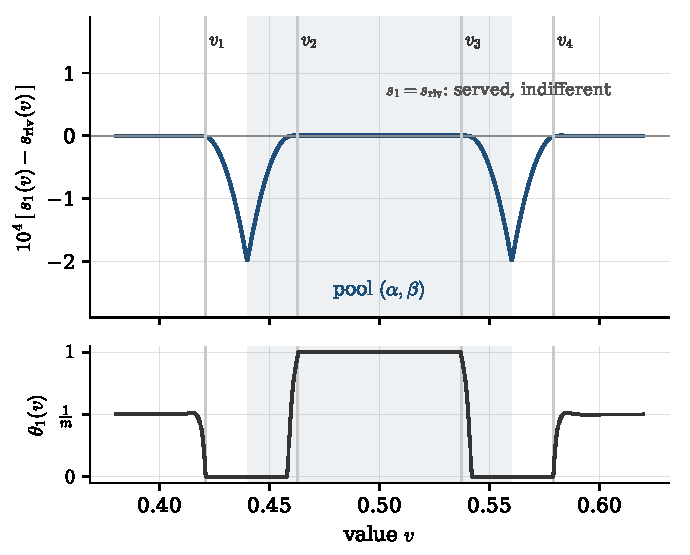
\includegraphics[width=0.66\linewidth]{figs/fig-band.pdf}
\caption{Equilibrium-solver output for continuation play after an interior pooling deviation: uniform $F$ on $[0,1]$, $\rho=0.1$, $m=n=2$, pool $(0.44,0.56)$. Top: surplus gap $s_1-s_{\mathrm{riv}}$, which vanishes off the band and on the served segment $(v_2,v_3)$, and is strictly negative on the outer segments. Bottom: seller $1$'s visit probability $\theta_1$, matching the analytical band points $(0.42,0.46,0.54,0.58)$ from Lemma~\ref{lem:band_detail} in Appendix~\ref{app:visits}.}
\label{fig:band}
\end{figure}

Figure~\ref{fig:band} illustrates the sorting pattern. A seller who pools $(\alpha,\beta)$ does not keep all the buyers he pools: types in $(v_1,\alpha)$ just below the pool face a higher winning probability at rivals and leave; types in $(\alpha,v_2)$ benefit locally from pooling ($\sigma'>0$) yet still visit rivals because the surplus deficit accumulated on $(v_1,\alpha)$ has not yet been recovered; and types in $(v_3,\beta)$ lose from pooling and also leave, creating a deficit that persists up to $v_4$. Only the middle fraction $1/m$ of the band visits seller $1$, and it does so exclusively so that rivals' effective distribution stays flat on $(v_2,v_3)$ and matches seller $1$'s flat pooled winning probability. At $n=2$, \eqref{eq:qstar} gives $q^*=\frac{\underline q+\bar q}{2}$ and the two outer segments carry equal quantile mass; for $n>2$, this holds up to an $O(\Delta^2)$ error in the band mass $\Delta=F(v_4)-F(v_1)$ (explicit endpoint formulas and top-reaching bands with $v_4=1$ are recorded in Lemma~\ref{lem:band_detail} in Appendix~\ref{app:visits}).

%%%%%%%%%%%%%%%%%%%%%%%%%%%%%%%%%%%%%%%%%%%%%%%%%%%%%%%%%%%%%%%%%%%%
\section{The Cournot Representation and Covered Markets} \label{sec:cournot}
%%%%%%%%%%%%%%%%%%%%%%%%%%%%%%%%%%%%%%%%%%%%%%%%%%%%%%%%%%%%%%%%%%%%

We now translate the continuation after any unilateral deviation into quantity coordinates. Doing so expresses a competing auctioneer's revenue as a weighted integral of Cournot oligopoly revenues. All proofs for Sections~\ref{sec:cournot}--\ref{sec:binding} appear in Appendix~\ref{app:interim}.

\subsection{Quantity Paths and Border's Condition}

Let rivals post $\SPA(\rho)$ for any $\rho\in[0,1)$, whether slack ($\rho<a$) or binding ($\rho\ge a$), and let seller $1$ deviate to any $\bmm_1=(r_1,\cP)\in\M$. Write $\underline r:=\min\{r_1,\rho\}$ and consider the unique localized SR continuation of Proposition~\ref{prop:unique}. For each type $v\in[\max\{\underline r,a\},1]$, define the upper-tail quantities
\[
T(v) := 1 - F_1(v), \qquad q(v) := 1 - F_{\mathrm{riv}}(v),
\]
representing the mass of buyers with values above $v$ who visit seller $1$ and each rival, respectively. Since every buyer above $\max\{\underline r,a\}$ visits some seller,
\[
T(v) + (m-1)q(v) = 1 - F(v).
\]
Let $P(z):=F^{-1}(1-z)$ denote the inverse demand curve on $[0,1]$, so $v=P\bigl(T(v)+(m-1)q(v)\bigr)$ is the market-clearing price when seller $1$ supplies $T$ and each rival supplies $q$, and let
\[
\Pi(t,q) := t\,P\bigl(t + (m-1)q\bigr)
\]
be the revenue of a Cournot oligopolist producing $t$ against $m-1$ rivals producing $q$. Along the symmetric diagonal $t=q$ (total quantity $z=mq$), a Cournot seller's marginal revenue is
\[
\partial_t \Pi(q,q) = P(mq) + q P'(mq) = P(z) - \frac{z}{m f(P(z))} = \psi_m\bigl(P(mq)\bigr).
\]

As $v$ falls from $1$ to $\max\{\underline r,a\}$, the pair $(q(v),T(v))$ traces a nondecreasing path from $(0,0)$ to the final traffic levels $(q_0,t_0)$, where $t_0+(m-1)q_0=1$ if $\underline r\le a$ and $t_0+(m-1)q_0\le 1$ if $\underline r>a$. We write $t(q)$ for seller $1$'s quantity as a function of a rival's quantity $q\in[0,q_0]$ (vertical jumps in $T$ at constant $q$ correspond to segments visited exclusively by seller $1$, and do not affect Lebesgue integrals in $q$). At the symmetric profile $\SPA(\rho)^m$, buyers split evenly and the path is the diagonal $t(q)=q$. Figure~\ref{fig:paths} shows schematic quantity paths for four basic deviations.

\begin{figure}[t]
\centering
\qpathpanel{Reserve increase}{\draw[accent,line width=1.2pt] (0,0)--(0.36,0.36)--(0.62,0.36);}{sheds low types}\hfill
\qpathpanel{Reserve cut}{\draw[accent,line width=1.2pt] (0,0)--(0.42,0.42)--(0.42,0.58);}{captures low types}\hfill
\qpathpanel{Interior pool}{\draw[accent,line width=1.2pt] (0,0)--(0.18,0.18)--(0.30,0.18)--(0.30,0.46)--(0.46,0.46)--(0.50,0.50);}{staircase}\hfill
\qpathpanel{Asking price}{\draw[accent,line width=1.2pt] (0,0)--(0.32,0.32)--(0.42,0.32)--(0.42,0.58);}{pool at reserve}
\caption{Schematic quantity paths $t(q)$ in the $(q,t)$-plane (illustrated for $m=2$, where $t+q\le 1$). The top of the market ($v=1$) lies at the origin $(0,0)$, and $\SPA(\rho)^m$ traces the dashed diagonal $t(q)=q$.}
\label{fig:paths}
\end{figure}

Let $W(dq):=n(n-1)(1-q)^{n-2}\,dq$ denote $n$ times the density of the maximum of $n-1$ independent draws from a uniform distribution on $[0,1]$.

\begin{proposition}[\textsc{Quantity-Path Representation}]\label{prop:path}
Suppose rivals post $\SPA(\rho)$ with $\rho\in[0,1)$, and seller $1$ deviates to any $(r_1,\cP)\in\M$. In the unique SR continuation, seller $1$'s revenue is
\begin{equation}\label{eq:pathrev}
R_1 = n\rho\,t_0(1-q_0)^{n-1} + \int_0^{q_0} \Pi\bigl(t(q),q\bigr)\,W(dq) - \ell,
\end{equation}
where $\ell\ge 0$ is the extra rent left to strictly preferring buyers at the bottom of the market ($\ell=0$ whenever all of seller $1$'s customers are indifferent). Moreover, Border's feasibility constraint \eqref{eq:border} together with sequential rationality implies
\begin{equation}\label{eq:borderq}
\int_0^q \bigl(t(u)-u\bigr)(1-u)^{n-2}\,du \le 0 \qquad \text{for all } q\in[0,q_0].
\end{equation}
\end{proposition}

Proposition~\ref{prop:path} follows from integrating the rent-extraction formula \eqref{eq:payoffs} by parts in $q$ (Appendix~\ref{app:interim}, where Lemma~\ref{lem:path_detail} defines $\ell$ explicitly and records the exact bottom-boundary identities used in the covered-market proof). Every customer who is indifferent between seller $1$ and a rival keeps the surplus she would earn at a rival, which depends only on the rival's quantity schedule $q(\cdot)$. Subtracting that surplus from total value created at seller $1$ leaves the Cournot rectangle $\Pi(t(q),q)$ at each rival quantity level $q$, weighted by $W(dq)$, plus the baseline revenue $n\rho\,t_0(1-q_0)^{n-1}$ collected at the rivals' reserve. The family of inequalities \eqref{eq:borderq} reflects Border's constraint \eqref{eq:border} in quantity coordinates: on weighted average, a seller with one unit cannot allocate more than his rivals to the highest types in the market.

\subsection{Interior Pools}

Call a finite collection $\cP$ of pooling intervals \emph{interior} (given rivals at $\SPA(\rho)$) if in the unique continuation of $(\rho,\cP)$ against $m-1$ rivals posting $\SPA(\rho)$, the split remains uniform near the bottom of the market---that is, every band lies strictly above $\max\{\rho,a\}$ (possibly reaching $1$ at the top).\footnote{Interiority is a property of the induced continuation rather than of the pool endpoints alone: a very wide pool with $\alpha>\max\{\rho,a\}$ can induce a band that touches the bottom of the market.} For any interior collection, all of seller $1$'s customers are indifferent ($\ell=0$) and his total traffic equals a rival's ($t_0=q_0=\frac{1-F(\rho)}{m}$). Subtracting \eqref{eq:pathrev} at the symmetric diagonal immediately yields an exact representation for any collection of interior pools, whether their bands are disjoint or merge into a single maximal non-uniform interval (a \emph{merged band}).

\begin{theorem}[\textsc{Interior Pools and Cournot's Condition}]\label{thm:cournot}
Suppose rivals post $\SPA(\rho)$ for some $\rho\in[0,1)$, and seller $1$ posts $(\rho,\cP)\in\M$ for a finite collection $\cP$ of interior pooling intervals. Let $q_{\rho}:=\frac{1-F(\rho)}{m}$.
\begin{enumerate}[(i)]
\item The exact change in seller $1$'s revenue is
\begin{equation}\label{eq:cournotD}
D = \int_0^{q_{\rho}} \Bigl[\Pi\bigl(t(q),q\bigr) - \Pi(q,q)\Bigr]\,W(dq),
\end{equation}
where $t(q)$ is a nondecreasing staircase with $t(q)=q$ off the bands, and on each merged band $[\underline q,\bar q]$ satisfies
\begin{equation}\label{eq:zeromean}
\int_{\underline q}^{\bar q}(1-q)^{n-2}\bigl(t(q)-q\bigr)\,dq = 0.
\end{equation}
\item If Cournot's marginal revenue $\psi_m(v)=v-\frac{1}{m}\frac{1-F(v)}{f(v)}$ is nondecreasing on the union of the bands (in particular, if it is nondecreasing on $[\max\{\rho,a\},1]$), then $D\le 0$.
\end{enumerate}
\end{theorem}

The argument for part~(ii) is short once the representation is in hand. When $\psi_m$ is nondecreasing, Cournot marginal revenue $\mathrm{MR}(z):=\psi_m(P(z))$ is nonincreasing in $z$. Because $P'(z)<0$, for any $s,q$ with $z=s+(m-1)q$ we have $\partial_t\Pi(s,q)=\mathrm{MR}(z)+\frac{m-1}{m}(s-q)P'(z)$, which lies below $\mathrm{MR}(mq)$ for $s\ge q$ and above it for $s\le q$. Integrating $s$ from $q$ to $t$ gives the diagonal tangent bound
\begin{equation}\label{eq:tangent_body}
\Pi(t,q) - \Pi(q,q) \le \psi_m\bigl(P(mq)\bigr)\,\bigl(t - q\bigr).
\end{equation}
Writing $\mathcal E(q):=(n-1)\int_0^q (t(u)-u)(1-u)^{n-2}\,du$, we have $\mathcal E\le 0$ everywhere by \eqref{eq:borderq}, and Border's condition binds off the bands, so $\mathcal E$ vanishes at both ends of every merged band $[\underline q,\bar q]$ (which yields \eqref{eq:zeromean}). Substituting \eqref{eq:tangent_body} into \eqref{eq:cournotD} and integrating by parts on each merged band gives
\[
D \le n\sum \int_{\underline q}^{\bar q} \psi_m\bigl(P(mq)\bigr)\,d\mathcal E(q) = -n\sum \int_{\underline q}^{\bar q} \mathcal E(q)\,d\psi_m\bigl(P(mq)\bigr) \le 0,
\]
since $q\mapsto\psi_m(P(mq))$ is nonincreasing. Intuitively, a pool causes the seller to supply too little against the top of each band (where marginal revenue is high) and too much against the bottom (where marginal revenue is low), with zero net change in weighted supply; under monotone Cournot marginal revenue, such misadjustments cannot pay.

The same tangent-and-Border argument applies to any deviation with $r_1\ge\rho$ that leaves seller $1$ with weakly less traffic than a rival, whether rivals' reserve is slack or binding.

\begin{corollary}[\textsc{A Smaller Seller Does Not Pool}]\label{cor:smaller}
Suppose rivals post $\SPA(\rho)$ for some $\rho\in[0,1)$ and $\psi_m$ is nondecreasing on $[\max\{\rho,a\},1]$. Any deviation $(r_1,\cP)\in\M$ with $r_1\ge\rho$ whose continuation leaves all of seller $1$'s customers indifferent and leaves him with weakly less traffic than a rival ($t_0\le q_0$) earns at most the revenue of the standard auction $\SPA(r)$ (with $r\ge\rho$) inducing the same traffic $t_0$.
\end{corollary}

\subsection{Equilibrium in Covered Markets}

We now turn to full equilibrium in a covered market ($a>0$). When sellers are restricted to second price auctions, \citeasnoun{virag2010competing} shows that among symmetric profiles with slack reserves $\rho<a$, only
\begin{equation}\label{eq:rhostar}
\rho^* = \frac{(n-1)\,a}{(m-1)^2 + n - 1} < a
\end{equation}
satisfies the first-order condition of the reserve game.\footnote{A reserve below $a$ excludes no buyer; it acts solely as the price paid by a buyer who happens to be alone at a seller. As Theorem~\ref{thm:bind} in Section~\ref{sec:binding} shows, no symmetric binding reserve $\rho\in[a,1]$ can be an equilibrium in $\M$, so $\SPA(\rho^*)^m$ is the unique symmetric equilibrium candidate among standard auctions.}

Our main positive result shows that Cournot's two conditions, monotone marginal revenue (no misallocation) and nonnegative marginal revenue at $a$ (no withholding), suffice for $\SPA(\rho^*)^m$ to be an equilibrium of $\Gamma$.

\begin{theorem}[\textsc{Covered Markets}]\label{thm:covered}
Suppose the market is covered ($a>0$). If $\psi_m$ is nondecreasing on $[a,1]$ and $\psi_m(a)\ge 0$ (equivalently, $a f(a)\ge\frac{1}{m}$), then $\SPA(\rho^*)^m$ is an equilibrium of $\Gamma$.
\end{theorem}

\begin{sketch}
Fix any deviation $(r_1,\cP)\in\M$ with quantity path $t(\cdot)$ ending at $(q_0,t_0)$, where $t_0+(m-1)q_0=1$. If $t_0\le\frac{1}{m}$ (the deviation loses traffic), a generalized tangent bound relative to the reserve-increase path $t^S(q)=\min\{q,t_0\}$ (equation~\eqref{eq:tangent_app} in Appendix~\ref{app:interim}) and integration by parts against \eqref{eq:borderq} show that the deviation earns no more than the reserve increase $\SPA(r)$ leaving traffic $t_0$. Differentiating the reserve-increase revenue $R^S(t_0)$ from \eqref{eq:pathrev} yields
\begin{align*}
\frac{1}{n}\frac{dR^S}{dt_0} &= \rho^*(m-2)(q_0-t_0)(1-q_0)^{n-2} \\
&\quad + (n-1)\int_{t_0}^{q_0}\Bigl[P\bigl(t_0+(m-1)q\bigr)+t_0 P'\bigl(t_0+(m-1)q\bigr)\Bigr](1-q)^{n-2}\,dq.
\end{align*}
Since $t_0\le \frac{z}{m}$ for $z=t_0+(m-1)q$ on $[t_0,q_0]$ and $P'<0$, the bracket is at least $\psi_m(P(z))\ge\psi_m(a)\ge 0$, so $R^S$ is nondecreasing on $[0,\frac{1}{m}]$ and every reserve increase loses.

If $t_0>\frac{1}{m}$ (the deviation gains traffic, so $q_0<\frac{1}{m}$), applying \eqref{eq:tangent_body} along the diagonal together with a covered-market lower bound on the capture rent $\ell$ (Lemma~\ref{lem:path_detail} in Appendix~\ref{app:interim}) bounds $R_1$ by the revenue of following the diagonal to $q_0$ and capturing the remaining buyers, less a Border convexity penalty. Comparing this bound to candidate revenue $R^*$ at $\rho^*$ reduces to the elementary inequality
\[
\frac{m-1}{m}(1-q_0)^n + \frac{1}{m}\bigl((m-1)q_0\bigr)^n \ge \Bigl(\frac{m-1}{m}\Bigr)^n,
\]
which holds by Jensen's inequality. See Appendix~\ref{app:interim}.
\end{sketch}

Theorem~\ref{thm:covered} requires no separate hypothesis that $\SPA(\rho^*)^m$ is an equilibrium of the reserve game: nonnegativity of $\psi_m$ on $[a,1]$ guarantees that $R^S(t_0)$ is globally nondecreasing on $[0,\frac{1}{m}]$, while the Case~2 bound for reserve cuts uses only $P\ge a$ (showing that reserve cuts never pay at $\rho^*$ in a covered market for any $F$). Thus $\psi_m\ge 0$ on $[a,1]$ alone suffices for $\SPA(\rho^*)^m$ to be an equilibrium of Vir\'ag's reserve game.

Because $\psi_m$ is strictly increasing whenever $\psi_1$ is nondecreasing, standard auctions can survive under competition even when a monopolist would pool.

\begin{example}[\textsc{A Non-Regular Distribution}]\label{ex:pareto}
Let $m=2$, and let buyer valuations follow a truncated Pareto (shifted Lomax) distribution on $[\frac{1}{2},1]$ with tail exponent $\frac{1}{2}$.\footnote{Specifically, $1-F(v)=\frac{S(v)-S(1)}{1-S(1)}$ on $[\frac{1}{2},1]$ with $S(v)=\bigl(1+198(v-\frac{1}{2})\bigr)^{-1/2}$ and $S(1)=\frac{1}{10}$; the worked-out calculation appears in Appendix~\ref{app:interim}.} Near the bottom of the support, Myerson's virtual valuation $\psi_1$ is positive yet strictly decreasing, so a monopolist serves those types and irons. Across the entire support, however, $\psi_2$ is strictly increasing and $\psi_2(\frac{1}{2})>0$. By Theorem~\ref{thm:covered}, both sellers posting $\SPA(\rho^*)$ with $\rho^*=\frac{n-1}{2n}$ is an equilibrium of $\Gamma$ for every $n\ge 2$.
\end{example}

%%%%%%%%%%%%%%%%%%%%%%%%%%%%%%%%%%%%%%%%%%%%%%%%%%%%%%%%%%%%%%%%%%%%
\section{Binding Reserves} \label{sec:binding}
%%%%%%%%%%%%%%%%%%%%%%%%%%%%%%%%%%%%%%%%%%%%%%%%%%%%%%%%%%%%%%%%%%%%

We now move to markets in which reserves bind ($\rho\ge a$), most notably when buyer values extend down to sellers' cost ($a=0$). Here the logic of Section~\ref{sec:cournot} reverses completely: no condition on $F$ rescues symmetric standard auctions, because competition itself creates a first-order incentive to pool buyers at the margin.

\subsection{Symmetric Profiles Fail via Asking Prices}

\begin{theorem}[\textsc{Symmetric Binding Reserves Fail}]\label{thm:bind}
Suppose a common reserve $\rho\in(0,1)$ binds ($\rho\ge a$). Then $\SPA(\rho)^m$ is not an equilibrium of $\Gamma$: deviating to the asking price $(\rho,\{(\rho,\beta)\})$ yields revenue gain
\begin{equation}\label{eq:askgain}
D = \frac{2n(m-1)}{m(m+3)}\,\rho\,A(\rho)^{n-1}\,\bigl(F(\beta)-F(\rho)\bigr) + o(\beta-\rho),
\end{equation}
which is strictly positive for every $\beta$ sufficiently close to $\rho$; in terms of seller $1$'s served pooled mass $e=\frac{4}{m+3}(F(\beta)-F(\rho))+o(\beta-\rho)$, equivalently $D=\frac{n(m-1)}{2m}\rho A(\rho)^{n-1}e+o(e)$. Moreover, at $\rho=1$ any lower reserve strictly raises revenue, and when $a=\rho=0$ a small reserve increase strictly raises revenue; hence no symmetric profile $\SPA(\rho)^m$ with $\rho\in[\max\{a,0\},1]$ is an equilibrium (in particular, none with $\rho\in[0,1]$ when $a=0$).
\end{theorem}

Why does an asking price strictly raise revenue at a binding reserve? Two forces combine.

First, capturing marginal traffic at a binding reserve yields a first-order profit. A buyer just above $\rho$ earns virtually zero surplus at every rival, so pooling a narrow interval $(\rho,\beta)$ lets seller $1$ serve an exclusive slice of mass $e$ just above $\rho$ at price $\rho$, while shedding a smaller mass of slightly higher types to rivals. To first order in $e$, the congestion effects on higher types cancel, leaving seller $1$ with a pure net-traffic profit $n\rho A(\rho)^{n-1}\cdot\frac{m-1}{2m}e$, proportional to his net traffic gain $\frac{m-1}{2m}e$.

Second, pooling is essential to hold that captured segment in place. If seller $1$ keeps reserve $\rho$ without pooling and tries to attract an exclusive slice of buyers just above $\rho$, the extra traffic congests his auction and lowers the winning probability of the lowest types near $\rho$ below his rivals' winning probability; those types defect back to rivals and capture unravels from below. Pooling $(\rho,\beta)$ equalizes winning probabilities across the captured segment, matching rivals' flat winning probability and keeping the captured buyers at seller $1$.

Figure~\ref{fig:dichotomy} contrasts the asking-price deviation at a binding reserve (first-order gain) against a covered market at the slack reserve $\rho^*$ (where buyers at $a$ already earn strictly positive surplus at every rival, eliminating the first-order gain).

\begin{figure}[t]
\centering
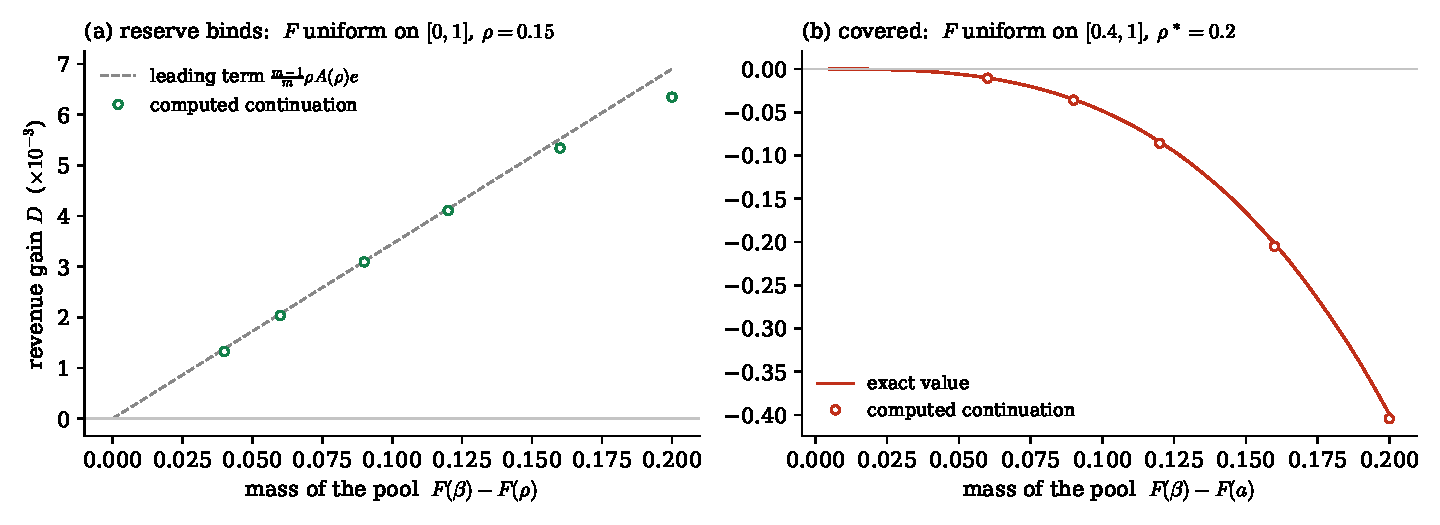
\includegraphics[width=\linewidth]{figs/fig-dichotomy.pdf}
\caption{Value of an asking price $(\rho,\{(\rho,\beta)\})$ at $m=n=2$ for uniform $F$. (a) Binding reserve ($F$ uniform on $[0,1]$, $\rho=0.15$): leading-order line from Theorem~\ref{thm:bind} alongside equilibrium-solver values. (b) Covered market ($F$ uniform on $[0.4,1]$, $\rho^*=0.2$): analytical revenue curve alongside solver values.}
\label{fig:dichotomy}
\end{figure}

\subsection{Asymmetric Reserves}

Theorem~\ref{thm:bind} rules out symmetric profiles of standard auctions with binding reserves. When $a=0$ and $m=2$, the reserve game has no symmetric pure equilibrium \citep{burguet}, though for regular $F$ and sufficiently large $n$ it admits a pure equilibrium in \emph{asymmetric} reserves $r_{L,n}<r_{H,n}$ whose reserves converge to distinct limits $0<r_L<r_H<1$ with $\psi_2(r_H)=0$ \citep{he2026}.

By Proposition~\ref{prop:pot}(ii), in any asymmetric duopoly profile $(\SPA(r_{L,n}),\SPA(r_{H,n}))$ with $r_{L,n}<r_{H,n}$, buyers in $(r_{L,n},w_n)$ visit seller $L$ exclusively while buyers above the indifference cutoff $w_n$ split evenly. Because buyers just above $r_{L,n}$ are already captive to $L$, neither seller can run the symmetric asking-price deviation of Theorem~\ref{thm:bind}. Nevertheless, asymmetric duopoly profiles with a high reserve where $\psi_1(r_H)<0$ also fail in $\M$ once $n$ is large: the low-reserve seller strictly profits by raising his reserve and adding a pool straddling $w_n$.

\begin{theorem}[\textsc{Asymmetric Reserves Fail for Large $n$}]\label{thm:asym}
Suppose $m=2$ and $a=0$. Consider any sequence of asymmetric profiles $\bigl(\SPA(r_{L,n}),\SPA(r_{H,n})\bigr)$ with $r_{L,n}\to r_L$ and $r_{H,n}\to r_H$ as $n\to\infty$, where $0\le r_L<r_H<1$ and $\psi_1(r_H)<0$. For all sufficiently large $n$, seller $L$ strictly increases his revenue by raising his reserve to some $v_{0,n}\in(r_{L,n},r_{H,n})$ and adding a single pooling interval straddling the indifference cutoff $w_n$.
\end{theorem}

For any regular distribution $F$, $\psi_1(r_H)<0$ means that $r_H$ lies strictly below the monopoly reserve. In particular, at the limiting asymmetric reserve equilibrium of \citeasnoun{he2026}, $\psi_2(r_H)=0$ implies $\psi_1(r_H)=-r_H<0$, so that equilibrium fails in $\M$ for every regular distribution once $n$ is sufficiently large. The economic motive echoes Theorem~\ref{thm:bind}: wherever a seller's exclusive buyers meet shared buyers at a type with negative monopoly virtual valuation, a narrow pool across the cutoff lets him raise his reserve on his captive block without losing the shared buyers near $w_n$ (Appendix~\ref{app:interim} gives the exact $O(1/n)$-scale construction and its closed-form limiting gain).

Two qualifications are worth noting. First, the revenue gains in both Theorem~\ref{thm:bind} (scaling as $A(\rho)^{n-1}$) and Theorem~\ref{thm:asym} (scaling as $(1-q_{w_n})^n$) are strictly positive at every finite $n$ yet vanish geometrically as $n\to\infty$, reflecting the rapid disappearance of market power near the bottom when buyers are plentiful. Second, Theorem~\ref{thm:asym} leaves open asymmetric profiles with $m\ge 3$, binding asymmetric reserves when $a>0$, and sequences whose reserves converge to a common limit ($r_L=r_H$) or to a limit with $\psi_1(r_H)\ge 0$. What equilibrium replaces standard auctions when reserves bind remains an open question.

%%%%%%%%%%%%%%%%%%%%%%%%%%%%%%%%%%%%%%%%%%%%%%%%%%%%%%%%%%%%%%%%%%%%
\section{Sharpness of Cournot's Condition} \label{sec:sharp}
%%%%%%%%%%%%%%%%%%%%%%%%%%%%%%%%%%%%%%%%%%%%%%%%%%%%%%%%%%%%%%%%%%%%

Theorem~\ref{thm:cournot} shows that monotonicity of $\psi_m$ rules out interior pooling for every number of buyers, and Theorem~\ref{thm:covered} extends this to full equilibrium in covered markets when $\psi_m(a)\ge 0$. We conclude our analysis by asking how sharp Cournot's monotonicity condition is across $n$, deferring the detailed propositions and proofs to Appendix~\ref{app:sharp}.

Under Assumption~\ref{a:two}, measure the curvature of demand by
\[
E(v) := -\frac{\bigl(1-F(v)\bigr)f'(v)}{f(v)^2}.
\]
Monotonicity of a weighted virtual valuation $v-\varpi\frac{1-F(v)}{f(v)}$ is equivalent to $E(v)\le 1+\frac{1}{\varpi}$; thus Myerson's regularity is $E\le 2$, while Cournot's condition is $E\le m+1$. Define the strictly smaller markup weight
\[
\varpi(m) := \frac{m+1}{m^2+2m-1} < \frac{1}{m},
\]
whose curvature threshold is $\bar X:=1+\frac{1}{\varpi(m)}=\frac{m(m+3)}{m+1}>m+1$.

\begin{theorem}[\textsc{Sharpness of Cournot's Condition}]\label{thm:sharp}
Impose Assumption~\ref{a:two}.
\begin{enumerate}[(i)]
\item \emph{Small pools at any fixed $n$.} Fix $n\ge 2$, rivals at $\SPA(\rho)$, and $v\in(\max\{\rho,a\},1)$. If $v-\varpi(m)\frac{1-F(v)}{f(v)}$ has strictly positive derivative at $v$ ($E(v)<\bar X$), then there exists $\bar\eta(n,v)>0$ such that every pooling deviation $(\rho,\{(\alpha,\beta)\})$ with $\alpha<v<\beta$ and $\beta-\alpha<\bar\eta(n,v)$ strictly lowers seller $1$'s revenue. Conversely, if it has strictly negative derivative at $v$ ($E(v)>\bar X$), then every sufficiently narrow pool containing $v$ strictly raises seller $1$'s revenue.
\item \emph{Many buyers.} For every $X>m+1$, there exists a covered-market distribution ($a>0$) satisfying Assumptions~\ref{a:one}--\ref{a:two} with $\psi_m(a)>0$ and $E\le X$ everywhere on $[a,1]$ such that, for every sufficiently large $n$, seller $1$ has an interior pooling deviation against $\SPA(\rho^*)^m$ that strictly raises his revenue. Thus $m+1$ is the largest upper bound on $E$ that rules out interior pooling (and supports covered-market equilibrium) for every $n$.
\end{enumerate}
\end{theorem}

\begin{figure}[t]
\centering
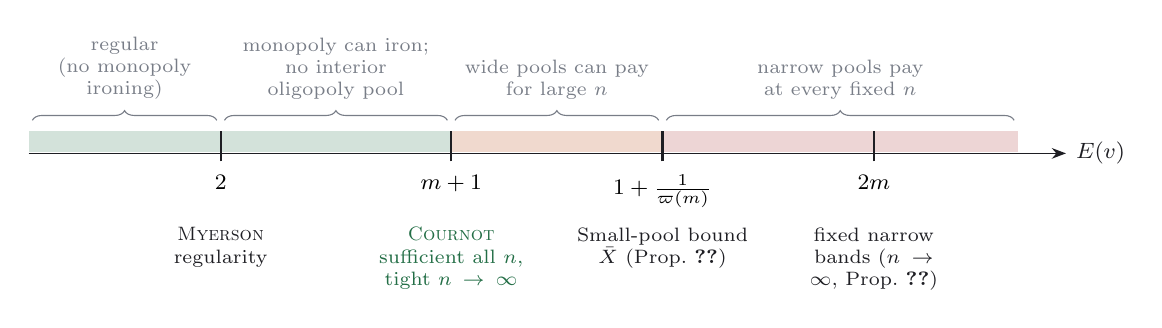
\begin{tikzpicture}[xscale=1.22]
  \draw[-{Stealth[length=1.8mm]},ink,line width=0.6pt] (0,0)--(10.8,0) node[right,font=\footnotesize]{$E(v)$};
  \fill[poscol,opacity=0.20] (0,0.02) rectangle (4.4,0.28);
  \fill[accent,opacity=0.22] (4.4,0.02) rectangle (6.6,0.28);
  \fill[negcol,opacity=0.20] (6.6,0.02) rectangle (10.3,0.28);
  \foreach \x/\l in {2/{2},4.4/{m+1},6.6/{1+\tfrac{1}{\varpi(m)}},8.8/{2m}} {
    \draw[ink,line width=0.8pt] (\x,-0.10)--(\x,0.28);
    \node[font=\footnotesize,below=2pt] at (\x,-0.08) {$\l$};
  }
  \draw[decorate,decoration={brace,amplitude=3.5pt},muted] (0.04,0.42)--(1.96,0.42)
    node[midway,above=4pt,font=\scriptsize,align=center,text width=2.2cm]{regular\\(no monopoly ironing)};
  \draw[decorate,decoration={brace,amplitude=3.5pt},muted] (2.04,0.42)--(4.36,0.42)
    node[midway,above=4pt,font=\scriptsize,align=center,text width=2.7cm]{monopoly can iron;\\no interior oligopoly pool};
  \draw[decorate,decoration={brace,amplitude=3.5pt},muted] (4.44,0.42)--(6.56,0.42)
    node[midway,above=4pt,font=\scriptsize,align=center,text width=2.5cm]{wide pools can pay\\for large $n$};
  \draw[decorate,decoration={brace,amplitude=3.5pt},muted] (6.64,0.42)--(10.26,0.42)
    node[midway,above=4pt,font=\scriptsize,align=center,text width=3.2cm]{narrow pools pay\\at every fixed $n$};
  \node[font=\scriptsize,align=center,anchor=north,text=ink,text width=2.1cm] at (2,-0.82) {\textsc{Myerson}\\regularity};
  \node[font=\scriptsize,align=center,anchor=north,text=poscol,text width=2.5cm] at (4.4,-0.82) {\textsc{Cournot}\\sufficient all $n$, tight $n\to\infty$};
  \node[font=\scriptsize,align=center,anchor=north,text=ink,text width=2.3cm] at (6.6,-0.82) {Small-pool bound\\$\bar X$ (Prop.~\ref{prop:smallpool})};
  \node[font=\scriptsize,align=center,anchor=north,text=ink,text width=2.4cm] at (8.8,-0.82) {fixed narrow\\bands ($n\to\infty$, Prop.~\ref{prop:manybuyers})};
\end{tikzpicture}
\caption{Curvature thresholds for interior pooling, with $E(v)=-\frac{(1-F(v))f'(v)}{f(v)^2}$ (note $E$ can be negative). At $m=1$ all four thresholds coincide at $2$; as $m\to\infty$ the three oligopoly thresholds diverge.}
\label{fig:curvature}
\end{figure}

Figure~\ref{fig:curvature} summarizes the curvature thresholds. Why does a gap open between the small-pool weight $\varpi(m)$ and Cournot's $1/m$? Along a narrow pooling staircase, the deviator's quantity jumps across the entire band while rivals' quantity moves linearly; expanding the Cournot integral \eqref{eq:cournotD} places $2:1$ weight on own-quantity concavity ($\partial_{tt}\Pi$, threshold $2m$) relative to the rival cross-effect ($\partial_{tq}\Pi$, threshold $m$), compared with Cournot's $1:1$ mix ($\partial_{tt}\Pi+\partial_{tq}\Pi$, threshold $m+1$). As $n$ grows large, however, the weighting measure $W(dq)\propto(1-q)^{n-2}\,dq$ concentrates at the top of any fixed band: the limits $d\to 0$ (band width) and $n\to\infty$ do not commute. Taking $d\to 0$ first at fixed $n$ yields $\bar X$ (with width threshold $\bar\eta(n,v)=O(1/n)$), whereas taking $n\to\infty$ first on a fixed narrow band yields the stricter own-concavity threshold $2m$; meanwhile, wide bands reaching near the top of the market compare the secant of $\Pi(\cdot,\underline q)$ against its tangent at $\underline q$, driving the sharpest uniform curvature bound down to Cournot's $m+1$ (Propositions~\ref{prop:smallpool}--\ref{prop:manybuyers} in Appendix~\ref{app:sharp}). Determining the exact critical curvature at a fixed finite $n\ge 2$ between $m+1$ and $\bar X$ remains open.

Finally, because $1/m$ vanishes as $m\to\infty$, interior misallocation is strictly a small-numbers phenomenon for any fixed smooth distribution: under Assumption~\ref{a:two}, $|E(v)|\le K/\underline f^2$, so for every $m\ge \lceil K/\underline f^2\rceil$ Cournot's marginal revenue $\psi_m$ is nondecreasing and every interior pool yields $D\le 0$ for all $n\ge 2$. Conversely, no uniform finite $m$ eliminates interior pooling across all smooth distributions: for any $m\ge 2$, the smooth truncated Pareto family $1-F(v)=\frac{S(v)-S(1)}{1-S(1)}$ with $S(v)=(1+c(v-a))^{-\alpha}$ and $S(1)=\frac{1}{2}$ has $E(a)=\frac{\alpha+1}{2\alpha}$, which exceeds $\bar X$ on an interval near $a$ once $\alpha<\frac{1}{2\bar X-1}$ and thus admits profitable narrow pools at every $n\ge 2$ by Theorem~\ref{thm:sharp}(i).

%%%%%%%%%%%%%%%%%%%%%%%%%%%%%%%%%%%%%%%%%%%%%%%%%%%%%%%%%%%%%%%%%%%%
\section{Related Literature} \label{sec:rellit}
%%%%%%%%%%%%%%%%%%%%%%%%%%%%%%%%%%%%%%%%%%%%%%%%%%%%%%%%%%%%%%%%%%%%

Our paper bridges monopolistic optimal auction theory \citep{myerson,bulow1989} and the literature on competing auctioneers. At the large-market limit, \citeasnoun{mcafee} shows that efficient second price auctions form an equilibrium when a deviating seller treats rivals' surpluses as fixed; \citeasnoun{peters} and \citeasnoun{peters1997} establish similar large-market efficiency results, while \citeasnoun{hernando2005} and \citeasnoun{ma2026} study convergence of finite-market equilibria. In finite markets, \citeasnoun{burguet} show that duopolists choosing reserves with $a=0$ have no symmetric pure equilibrium and construct a mixed one at $n=2$; \citeasnoun{virag2010competing} extends reserve competition to $m$ sellers, establishes the covered-market candidate \eqref{eq:rhostar}, and proves convergence of reserves to cost; and \citeasnoun{he2026} studies duopolists choosing between posted prices and second price auctions with reserves at $a=0$, showing that pure equilibria are in auctions and constructing the asymmetric-reserve equilibrium for regular distributions and large $n$ that Theorem~\ref{thm:asym} shows fails once pooling is allowed. \citeasnoun{virag} studies mechanism choice at $m=n=2$ with no withholding, finding conditions (increasing density and increasing reverse hazard rate) for standard auctions to survive. \citeasnoun{moldovanu} study competition in quantities followed by efficient auctions, and \citeasnoun{kim2015} recover efficiency in large markets via cheap talk.

Directed and competitive search models \citep[surveyed in][]{wright2021} also study buyers sorting across competing sellers, typically in large-market limits or with exogenous frictions; see \citeasnoun{burdett2001pricing}, \citeasnoun{eeckhout2010sorting}, and \citeasnoun{albrecht2014}, as well as \citeasnoun{lester2017}, who derive asking prices from inspection costs rather than strategic competition in a frictionless market. \citeasnoun{epstein1999} and \citeasnoun{peters2001common} analyze what is lost when competing mechanisms cannot condition on rivals' announcements.

Our Cournot interpretation connects to the conduct-parameter literature \citep{bresnahan1989,weyl2013} and competitive screening \citep{stole2007}. In competitive nonlinear pricing \citep{armstrong2001,rochet}, coverage eliminates screening distortions immediately even in duopoly, because brand preferences separate consumers across firms independently of their valuation type; when markets are not covered or vertical/informational frictions bind, distortions persist and shrink with competition \citep{yang2008,biais2000,chade2021}. Here sellers are homogeneous and buyers sort directly on valuations, so coverage alone does not eliminate misallocation without a curvature bound on $F$. Our weighted marginal revenue $\psi_m=(1-\frac{1}{m})v+\frac{1}{m}\psi_1$ also parallels redistributive mechanism design \citep{dworczak2021}, with the welfare weight emerging endogenously from competition rather than planner preferences, and relates to \citeasnoun{azevedo2019} on the rate at which incentive constraints vanish in large markets.

Methodologically, we rely on Border's reduced-form characterization \citep{border1,che2013,hartreny2015}, the extreme-point theory of majorization sets \citep{kleiner2021}, reduced-form implementation and ironing \citep{manelli2010,toikka2011}, and potential games \citep{monderer1996,vetta2002}. In the capacity-constrained pricing literature of \citeasnoun{kreps} and \citeasnoun{davidson}, rationing rules are exogenous; here the visit equilibrium endogenizes rationing while allowing sellers to choose mechanisms richer than posted prices. Finally, \citeasnoun{einav2018} document the shift from auctions to posted prices on eBay and attribute it to buyer hassle costs; our results isolate the purely strategic forces that can generate misallocation even without hassle costs.

%%%%%%%%%%%%%%%%%%%%%%%%%%%%%%%%%%%%%%%%%%%%%%%%%%%%%%%%%%%%%%%%%%%%
\section{Conclusion} \label{sec:conclude}
%%%%%%%%%%%%%%%%%%%%%%%%%%%%%%%%%%%%%%%%%%%%%%%%%%%%%%%%%%%%%%%%%%%%

We asked what replaces Myerson's regularity condition when finitely many sellers compete in mechanism design rather than being restricted to second price auctions. A seller's revenue is a weighted integral of Cournot oligopoly revenues (plus a boundary reserve term, net of any rents to strictly preferring buyers), so Cournot's marginal revenue $\psi_m(v)=v-\frac{1}{m}\frac{1-F(v)}{f(v)}$ governs interior misallocation. In covered markets, monotonicity and nonnegativity of $\psi_m$ suffice for symmetric standard auctions to form an equilibrium for every number of buyers. When reserves bind, competition creates a first-order motive to pool marginal buyers, overturning symmetric standard-auction profiles for every $n\ge 2$ and asymmetric duopoly profiles with $\psi_1(r_H)<0$ for all sufficiently large $n$. Finally, Cournot's curvature bound $E\le m+1$ cannot be weakened uniformly across $n$, whereas for narrow pools at any fixed $n$ the exact markup weight is $\varpi(m)<\frac{1}{m}$.

Several natural questions remain open:
\begin{enumerate}
\item \emph{Equilibrium when standard auctions fail.} Characterizing equilibria of $\Gamma$ when reserves bind, when a covered market has $\psi_m(a)<0$ or non-monotone $\psi_m$, or determining the exact curvature threshold at a fixed finite $n\ge 2$, remains open.
\item \emph{Multi-seller pooling continuations.} Proposition~\ref{prop:unique} establishes uniqueness of the visit continuation whenever one seller deviates to a mechanism with finitely many pools against rivals running standard auctions. Analyzing equilibria in which multiple sellers pool simultaneously requires extending continuation uniqueness to profiles where several sellers pool.
\item \emph{Beyond hierarchical mechanisms and single-seller visits.} Extending the strategy space beyond hierarchical mechanisms (for example, to mechanisms that condition on the realized number of visitors) and allowing buyers to participate in multiple auctions simultaneously are important directions for future work.
\end{enumerate}

\appendix
\counterwithin{lemma}{section}
\counterwithin{proposition}{section}
\counterwithin{remark}{section}
\counterwithin{figure}{section}
\counterwithin{table}{section}

%%%%%%%%%%%%%%%%%%%%%%%%%%%%%%%%%%%%%%%%%%%%%%%%%%%%%%%%%%%%%%%%%%%%
\section{Proofs for Section~\ref{sec:visits}} \label{app:visits}
%%%%%%%%%%%%%%%%%%%%%%%%%%%%%%%%%%%%%%%%%%%%%%%%%%%%%%%%%%%%%%%%%%%%

\subsection{Standard Auctions: A Potential Game}

\begin{lemma}[\textsc{Surplus Equals Marginal Contribution}]\label{lem:vcg}
For a finite set $S$ of buyers at $\SPA(r)$ with valuations $(v_k)_{k\in S}$, define $\widetilde W(S):=(\max_{k\in S}v_k-r)^+$ (with $\widetilde W(\emptyset):=0$). Under truthful bidding, the realized surplus of $i\in S$ equals $\widetilde W(S)-\widetilde W(S\setminus\{i\})$.
\end{lemma}
\begin{proof}
If $v_i<\max_{k\ne i}v_k$ or $v_i<r$, buyer $i$ neither wins nor alters the maximum above $r$, so both sides vanish. If $v_i\ge r$ equals $\max_{k\ne i}v_k$, buyer $i$ pays $v_i$ upon winning (zero surplus) and removing her leaves the maximum unchanged (both sides vanish). If $v_i\ge r$ is the unique maximum, her surplus is $v_i-\max\{r,\max_{k\ne i}v_k\}=(v_i-r)-(\max_{k\ne i}v_k-r)^+$.
\end{proof}

For possibly asymmetric visit strategies $(\theta^1,\dots,\theta^n)$, let $S_j$ be the random set of visitors at seller $j$, $\widetilde W_j(S_j):=(\max_{k\in S_j}v_k-r_j)^+$, $U_i(\theta^i,\theta^{-i})$ be buyer $i$'s ex-ante expected surplus, and $F_j^i(v):=1-\int_v^1\theta_j^i(u)f(u)\,du$. Define
\[
\widehat\Phi(\theta^1,\dots,\theta^n) := \EV{\textstyle\sum_{j=1}^m \widetilde W_j(S_j)} = \sum_{j=1}^m \int_{r_j}^1 \Bigl[1 - \prod_{i=1}^n F_j^i(v)\Bigr]\,dv,
\]
using the tail-integral identity for the maximum effective bid at seller $j$. Note that $\Phi(\theta)=\widehat\Phi(\theta,\dots,\theta)$ is \eqref{eq:pot}.

\begin{lemma}[\textsc{Exact Potential}]\label{lem:potential}
For every buyer $i$ and strategies $\theta^i,\tilde\theta^i,\theta^{-i}$, we have $U_i(\theta^i,\theta^{-i})-U_i(\tilde\theta^i,\theta^{-i})=\widehat\Phi(\theta^i,\theta^{-i})-\widehat\Phi(\tilde\theta^i,\theta^{-i})$, and $\widehat\Phi$ is affine in each coordinate.
\end{lemma}
\begin{proof}
By Lemma~\ref{lem:vcg}, conditional on valuations and rivals' visits, buyer $i$'s surplus is $\sum_j[\widetilde W_j(S_j)-\widetilde W_j(S_j\setminus\{i\})]$. Taking expectations gives $U_i(\theta^i,\theta^{-i})=\widehat\Phi(\theta^i,\theta^{-i})-C_{-i}(\theta^{-i})$, where $C_{-i}$ does not depend on $\theta^i$. Subtracting the same identity at $\tilde\theta^i$ gives the first claim; affinity is immediate because each $F_j^i$ is affine in $\theta^i$ and enters each product linearly.
\end{proof}

\begin{lemma}[\textsc{Derivative and Concavity}]\label{lem:deriv}
$\Phi$ is concave, with directional derivative
\[
\frac{d}{d\epsilon}\Phi\bigl(\theta+\epsilon(\tilde\theta-\theta)\bigr)\Big|_{\epsilon=0^+} = n\sum_{j=1}^m \int_a^1 \bigl(\tilde\theta_j(v)-\theta_j(v)\bigr)\,s_j(v)\,f(v)\,dv.
\]
If $\theta$ and $\theta'$ induce $F_j\ne F_j'$ on a positive-measure subset of $(r_j,1)$ for some $j$, then $\Phi(\frac{\theta+\theta'}{2})>\frac{1}{2}\Phi(\theta)+\frac{1}{2}\Phi(\theta')$.
\end{lemma}
\begin{proof}
Each $F_j$ is affine in $\theta$ and $y\mapsto -y^n$ is strictly concave on $[0,\infty)$, yielding concavity and the strict midpoint inequality. Writing $H_j(v):=\int_v^1(\tilde\theta_j(u)-\theta_j(u))f(u)\,du$,
\begin{align*}
\frac{d}{d\epsilon}\Bigl[-\int_{r_j}^1(F_j-\epsilon H_j)^n\,dv\Bigr]\Big|_{\epsilon=0^+}
&= n\int_{r_j}^1 F_j(v)^{n-1}H_j(v)\,dv \\
&= n\int_a^1\bigl(\tilde\theta_j(u)-\theta_j(u)\bigr)\,f(u)\Bigl[\int_{r_j}^{\max\{u,r_j\}} F_j(v)^{n-1}\,dv\Bigr]\,du
\end{align*}
by Fubini's theorem, and the inner bracket equals $s_j(u)$.
\end{proof}

\begin{proof}[Proof of Proposition~\ref{prop:pot}]
\emph{Sufficiency.} If $\theta$ maximizes $\Phi$ and buyer $i$ deviates to $\tilde\theta^i$, then by symmetry and coordinate-wise affinity of $\widehat\Phi$ the right derivative of $\epsilon\mapsto\Phi(\theta+\epsilon(\tilde\theta^i-\theta))$ at $0$ equals $n[\widehat\Phi(\tilde\theta^i,\theta,\dots,\theta)-\widehat\Phi(\theta,\dots,\theta)]\le 0$. By Lemma~\ref{lem:potential}, no buyer can profitably deviate, so $\theta$ is SR.

\emph{Necessity.} If $\theta$ is SR, then $\sum_j\tilde\theta_j(v)s_j(v)\le\max_k s_k(v)=\sum_j\theta_j(v)s_j(v)$ for almost every $v$, so every directional derivative of the concave functional $\Phi$ at $\theta$ is nonpositive by Lemma~\ref{lem:deriv}. Hence $\theta$ maximizes $\Phi$.

\emph{Existence and uniqueness.} Equip $\Theta:=\{\theta:[a,1]\to\Delta^m\text{ measurable}\}$ with the weak-$*$ topology of $L^\infty([a,1],\Re^m)$; it is convex, compact, and metrizable. If $\theta^\ell\to\theta$, then $F_j^\ell\to F_j$ pointwise and hence uniformly by equicontinuity ($|F_j^\ell(v)-F_j^\ell(v')|\le|F(v)-F(v')|$), so $\Phi(\theta^\ell)\to\Phi(\theta)$ by dominated convergence. Thus $\Phi$ attains a maximum on $\Theta$. If two maximizers differed in $F_j$ on a positive-measure subset of $(r_j,1)$, their midpoint would achieve strictly higher $\Phi$ by Lemma~\ref{lem:deriv}, a contradiction.

\emph{Part~(i).} Under a common reserve $\rho$, the uniform split makes all surpluses $s_j$ identical, so it is SR, and uniqueness gives $F_j=A$ on $[\rho,1]$.

\emph{Part~(ii).} Suppose first $r_1>\rho$, and consider the indifference equation
\begin{equation}\label{eq:w}
(w - r_1)\,A(w)^{n-1} = \int_\rho^w F_{\mathrm{riv}}(v;w)^{n-1}\,dv, \qquad F_{\mathrm{riv}}(v;w) := A(w) - \frac{F(w)-F(v)}{m-1}.
\end{equation}
Let $h(w):=(w-r_1)A(w)^{n-1}-\int_\rho^w F_{\mathrm{riv}}(v;w)^{n-1}\,dv$. On $[r_1,\max\{r_1,a\}]$, $F\equiv 0$ so $F_{\mathrm{riv}}(v;w)\equiv A(a)=1-\frac{1}{m}$, hence $h(w)=(\rho-r_1)(1-\frac{1}{m})^{n-1}<0$. For $w>\max\{r_1,a\}$, since $F_{\mathrm{riv}}(w;w)=A(w)$ and $\partial_w F_{\mathrm{riv}}(v;w)=-\frac{f(w)}{m(m-1)}<0$,
\[
h'(w) = (w-r_1)(n-1)A(w)^{n-2}\frac{f(w)}{m} + (n-1)\int_\rho^w F_{\mathrm{riv}}(v;w)^{n-2}\frac{f(w)}{m(m-1)}\,dv > 0.
\]
Hence \eqref{eq:w} has a unique solution $w\in(\max\{r_1,a\},1]$ by the intermediate value theorem whenever $h(1)\ge 0$; otherwise $h<0$ on $[r_1,1]$ and we set $w=1$. If $w<1$, the split assigning types below $w$ symmetrically to rivals and types above $w$ uniformly to all $m$ sellers yields $F_j=A$ above $w$; below $w$, $s_1$ is linear with slope $A(w)^{n-1}$ while $s_{\mathrm{riv}}'=F_{\mathrm{riv}}^{n-1}\le A(w)^{n-1}$ and $s_1(w)=s_{\mathrm{riv}}(w)$, so $s_{\mathrm{riv}}\ge s_1$ below $w$, confirming SR. If $w=1$, every type strictly prefers a rival and seller $1$ receives no traffic. Since $h$ is continuous in $(w,r_1)$, strictly increasing in $w$ above $\max\{r_1,a\}$, and strictly decreasing in $r_1$, $w(r_1)$ is continuous and nondecreasing in $r_1$.

When $r_1<\rho$, seller $1$ captures buyers below the cutoff exclusively, so $F_1(v;w):=A(w)-(F(w)-F(v))$ on $[r_1,w]$ and the indifference equation becomes
\begin{equation}\label{eq:w_rev}
(w - \rho)\,A(w)^{n-1} = \int_{r_1}^w F_1(v;w)^{n-1}\,dv.
\end{equation}
Writing $\tilde h(w):=(w-\rho)A(w)^{n-1}-\int_{r_1}^w F_1(v;w)^{n-1}\,dv$, we have $\tilde h(\max\{\rho,a\})<0$ and $\partial_w F_1(v;w)=-\frac{m-1}{m}f(w)<0$, so $\tilde h'(w)>0$ for all $w>\max\{\rho,a\}$. The identical argument yields a unique cutoff $w\in(\max\{\rho,a\},1]$ that is continuous and nonincreasing in $r_1$.
\end{proof}

\subsection{Uniqueness and Band Structure}

We pair Proposition~\ref{prop:unique} with the finer sub-interval properties used in subsequent proofs.

\begin{lemma}[\textsc{Sub-Interval Structure}]\label{lem:loc_detail}
In the unique SR continuation of Proposition~\ref{prop:unique}, each maximal non-uniform interval above $\max\{r_1,\rho,a\}$ is a finite union of sub-intervals with constant $\theta_1\in\{0,1\}$. Moreover, every sub-interval on which seller $1$'s customers are indifferent and visit him exclusively lies inside a single pool, at most one per pool.
\end{lemma}

\begin{proof}[Proof of Proposition~\ref{prop:unique} and Lemma~\ref{lem:loc_detail}]
\emph{Existence for any profile in $\M^m$.} Equip $\Theta:=\{\theta:[a,1]\to\Delta^m\text{ measurable}\}$ with the weak-$*$ topology of $L^\infty([a,1],\Re^m)$; it is convex, compact, and metrizable. If $\theta^\ell\to\theta$, then $F_j^\ell\to F_j$ pointwise and hence uniformly by equicontinuity ($|F_j^\ell(v)-F_j^\ell(v')|\le|F(v)-F(v')|$). Because allocations \eqref{eq:poolalloc} depend continuously on effective distributions (and their values at pool endpoints), surpluses $s_j(\cdot;\theta^\ell)$ converge uniformly to $s_j(\cdot;\theta)$. The best-response correspondence
\[
B(\theta):=\Bigl\{\theta'\in\Theta:\int_a^1\sum_{j=1}^m\theta_j'(v)s_j(v;\theta)f(v)\,dv=\int_a^1\max_{j} s_j(v;\theta)f(v)\,dv\Bigr\}
\]
is nonempty (assigning each type to the lowest-indexed maximizing seller), convex, and closed-graph. By \citeasnoun{glicksberg1952}, $B$ has a fixed point, which is SR.

Now suppose rivals post $\SPA(\rho)$ with $\rho\in[0,1)$ and seller $1$ posts $(r_1,\cP)\in\M$. Set $\underline r:=\min\{r_1,\rho\}$ and $\bar r:=\max\{r_1,\rho\}$. Every buyer visits some seller, so $\sum_j(1-F_j)=1-F$ on $[a,1]$; each $F_j$ is absolutely continuous with $F_j'=\theta_j f$, and each $s_j$ is absolutely continuous with $s_j'=x_j$. For a rival, $x_j=0$ below $\rho$ and $x_j=F_j^{n-1}$ above $\rho$. For seller $1$, $x_1=0$ below $r_1$, $x_1=F_1^{n-1}$ above $r_1$ off $\bigcup\cP$, and on each pool $(\alpha_i,\beta_i)\in\cP$ we have $x_1=\bar x_i=g(F_1(\alpha_i),F_1(\beta_i))$, where
\[
g(y,z) := \frac{1}{z-y}\int_y^z u^{n-1}\,du \quad (y<z), \qquad g(y,y):=y^{n-1}.
\]
Note that $g$ is continuous and strictly increasing in $(y,z)$, and since $y^{n-1}\le g(y,z)\le z^{n-1}$, $x_1$ is nondecreasing on $[0,1]$ (including across pool boundaries). Order the finitely many pools as $(\alpha_1,\beta_1),\dots,(\alpha_{\mathcal N},\beta_{\mathcal N})$ with $r_1\le\alpha_1<\beta_1\le\cdots\le\alpha_{\mathcal N}<\beta_{\mathcal N}\le 1$. Almost-everywhere statements below are with respect to $F$.

\emph{(i) Rival symmetry.} Fix an SR continuation and two rivals $j,k$. Set $H:=F_j-F_k$ and $S:=s_j-s_k$. By sequential rationality, $(\theta_j-\theta_k)S\ge 0$ a.e., so $\int_\rho^1 S\,dH=\int_\rho^1(\theta_j-\theta_k)Sf\,dv\ge 0$. Since $H(1)=0$, $S(\rho)=0$, and $S'=F_j^{n-1}-F_k^{n-1}$ on $[\rho,1]$, integration by parts gives
\[
0 \le \int_\rho^1 S\,dH = -\int_\rho^1 (F_j-F_k)(F_j^{n-1}-F_k^{n-1})\,dv \le 0.
\]
Since the integrand is continuous and nonnegative, $F_j=F_k=:F_{\mathrm{riv}}$ on $[\rho,1]$, giving common $x_{\mathrm{riv}}$ and $s_{\mathrm{riv}}$ there. Adding up yields $F_{\mathrm{riv}}=1-\frac{F_1-F}{m-1}$ on $[\rho,1]$.

\emph{(ii) Uniqueness.} Let $\sigma:=s_1-s_{\mathrm{riv}}$ on $[\underline r,1]$, so $\sigma(\underline r)=0$. Sequential rationality requires $\theta_1>0\implies\sigma\ge 0$ and $\theta_1<1\implies\sigma\le 0$ a.e. If $r_1<\rho$, every type $v\in(\max\{r_1,a\},\rho)$ has $F_1(v)\ge F(v)>0$, hence $x_1(v)>0$ and $s_1(v)>0=s_{\mathrm{riv}}(v)$, so $\theta_1=1$ a.e.\ on $(\max\{r_1,a\},\rho)$. Thus $F_1'=f$ a.e.\ on $[\underline r,\rho]$ in every SR continuation.

Compare two SR continuations (denoting the second with tildes) and set $\Delta F:=\tilde F_1-F_1$, $\Delta\sigma:=\tilde\sigma-\sigma$, and $\Delta\bar x_i:=\tilde{\bar x}_i-\bar x_i$. Both $\Delta F$ and $\Delta\sigma$ are absolutely continuous with $\Delta F(1)=0$ and $\Delta\sigma(\underline r)=0$, and satisfy five properties:
\begin{enumerate}[(a)]
\item $\Delta F'=(\tilde\theta_1-\theta_1)f$ a.e., so $\Delta F$ is constant on $[0,a]$ and on $[\underline r,\rho]$.
\item For a.e.\ type, $\Delta\sigma>0\implies\Delta F'\ge 0$ and $\Delta\sigma<0\implies\Delta F'\le 0$. (If $\tilde\theta_1<\theta_1$, then $\theta_1>0$ and $\tilde\theta_1<1$, so $\sigma\ge 0\ge\tilde\sigma$.)
\item On $(\underline r,1]$ off the pools, $\Delta\sigma'$ has the strict sign of $\Delta F$: wherever $\Delta F>0$, seller $1$'s allocation is strictly higher in the second continuation above $r_1$ and a rival's is strictly lower above $\rho$ (since $\tilde F_{\mathrm{riv}}-F_{\mathrm{riv}}=-\frac{\Delta F}{m-1}$), and every point above $\underline r$ exceeds $r_1$ or $\rho$.
\item On pool $(\alpha_i,\beta_i)$, $\Delta\sigma'=\Delta\bar x_i+\varphi$ a.e., where $\varphi:=x_{\mathrm{riv}}-\tilde x_{\mathrm{riv}}$ satisfies $|\varphi|\le\frac{n-1}{m-1}|\Delta F|$, vanishes below $\rho$, and above $\rho$ has the sign of $\Delta F$.
\item By monotonicity of $g$, $\Delta\bar x_i>0$ if $\Delta F(\alpha_i)\ge 0$ and $\Delta F(\beta_i)\ge 0$ with one strict; $\Delta\bar x_i<0$ in the mirror case; and $\Delta\bar x_i=0$ if both vanish.
\end{enumerate}

Call $(\Delta F,\Delta\sigma)$ \emph{positive} at $v$ if $\Delta F(v)>0$ and $\Delta\sigma(v)\ge 0$, \emph{strictly positive} if both are strict, \emph{negative} / \emph{strictly negative} symmetrically, \emph{signed} if it is positive or negative, and \emph{at rest} if both vanish. Each step below has a mirror image by swapping the two continuations.

\emph{Step 1 (gaps preserve sign).} Suppose $[u_1,u_2]$ meets no pool and $(\Delta F,\Delta\sigma)$ is positive at $u_1$. Let $c:=\sup\{v\le u_2:\Delta F>0\text{ on }[u_1,v]\}$. By (c), $\Delta\sigma$ strictly increases on $[u_1,c)$, so $\Delta\sigma>0$ on $(u_1,c)$; by (b), $\Delta F$ is nondecreasing on $[u_1,c)$, so $\Delta F(c)\ge\Delta F(u_1)>0$. Thus $c=u_2$, and the pair is strictly positive at $u_2$ if $u_2>u_1$.

\emph{Step 2 (pools cannot bring a signed pair to rest).} Suppose $(\Delta F,\Delta\sigma)$ is positive at $\alpha_i$.
If $\Delta\bar x_i\ge 0$, let $c:=\sup\{v\le\beta_i:\Delta F>0\text{ on }[\alpha_i,v]\}$. By (d), $\Delta\sigma'=\Delta\bar x_i+\varphi\ge 0$ on $[\alpha_i,c)$, strictly above $\rho$, so $\Delta\sigma>0$ on $(\max\{\alpha_i,\rho\},c)$ and $\Delta F$ is nondecreasing there by (b); on $[\alpha_i,\rho]$, $\Delta F$ is constant by (a). Hence $\Delta F(c)\ge\Delta F(\alpha_i)>0$, so $c=\beta_i$, $\Delta F(\beta_i)>0$, $\Delta\bar x_i>0$ by (e), and $\Delta\sigma'\ge\Delta\bar x_i>0$, leaving the pair strictly positive at $\beta_i$.
If instead $\Delta\bar x_i<0$, then $\Delta F(\beta_i)<0$ by (e). Let $z_0$ be the largest zero of $\Delta F$ on $[\alpha_i,\beta_i]$, so $\Delta F<0$ on $(z_0,\beta_i]$ and $z_0\ge\max\{\rho,a\}$ by (a). On $(z_0,\beta_i)$, $\Delta\sigma'=\Delta\bar x_i+\varphi<0$. If $\Delta\sigma$ remained positive throughout $(z_0,\beta_i)$, then $\Delta F$ would be nondecreasing there by (b), contradicting $\Delta F(z_0)=0>\Delta F(\beta_i)$. Thus $\Delta\sigma$ turns nonpositive before $\beta_i$ and is strictly negative at $\beta_i$.

\emph{Step 3 (from rest across a gap).} Suppose $[u_1,u_2]$ meets no pool and $(\Delta F,\Delta\sigma)$ is at rest at $u_1$. If $\Delta F(v_0)>0$ for some $v_0\in(u_1,u_2]$, let $J=(y_1,y_2)$ be the maximal interval in $[u_1,u_2]$ containing $v_0$ on which $\Delta F>0$, so $\Delta F(y_1)=0$. By (c), $\Delta\sigma$ strictly increases on $J$. If $\Delta\sigma(s)<0$ for some $s\in J$, then $\Delta\sigma<0$ on $(y_1,s]$, making $\Delta F$ nonincreasing there and contradicting $\Delta F(s)>0=\Delta F(y_1)$. Thus $\Delta\sigma>0$ on $J$, so $\Delta F$ is nondecreasing on $J$, forcing $y_2=u_2$ and leaving the pair strictly positive at $u_2$. By symmetry, if $\Delta F$ is not identically zero on $[u_1,u_2]$, the pair is strictly signed at $u_2$; if $\Delta F\equiv 0$, then $\Delta\sigma\equiv 0$ by (c).

\emph{Step 4 (from rest across a pool).} Suppose the pair is at rest at $\alpha_i$. If $\Delta F(\beta_i)>0$, then $\Delta\bar x_i>0$ by (e). If $\Delta F$ ever turned negative on $(\alpha_i,\beta_i)$, let $p_0:=\inf\{v\in(\alpha_i,\beta_i):\Delta F(v)<0\}$. Then $\Delta F(p_0)=0$ and $\Delta F\ge 0$ on $[\alpha_i,p_0]$, so $\Delta\sigma(p_0)\ge 0$ by (d). Because $|\varphi|\le\frac{n-1}{m-1}|\Delta F|$ and $\Delta F(p_0)=0$, we have $\Delta\sigma'\ge\frac{1}{2}\Delta\bar x_i>0$ near $p_0$, forcing $\Delta\sigma>0$ and hence $\Delta F\ge 0$ on $(p_0,p_0+\epsilon)$, contradicting the definition of $p_0$. Thus $\Delta F\ge 0$ and $\Delta\sigma'\ge\Delta\bar x_i>0$ throughout, leaving the pair strictly positive at $\beta_i$. The case $\Delta F(\beta_i)<0$ is symmetric. Finally, if $\Delta F(\beta_i)=0$, then $\Delta\bar x_i=0$ by (e) and $\Delta\sigma'=\varphi$. Any maximal interval $J=(y_1,y_2)\subset(\alpha_i,\beta_i)$ where $\Delta F>0$ has $y_1\ge\max\{\rho,a\}$ by (a) and $\Delta F(y_1)=\Delta F(y_2)=0$, yielding the same contradiction as Step~3. Hence $\Delta F=\Delta\sigma=0$ on $[\alpha_i,\beta_i]$.

\emph{Step 5.} The points $\underline r\le\alpha_1<\beta_1\le\cdots\le\alpha_{\mathcal N}<\beta_{\mathcal N}\le 1$ partition $[\underline r,1]$ into finitely many gaps and pools. At $\underline r$, $\Delta\sigma(\underline r)=0$, so the pair starts either at rest or signed; Steps~1--4 map $\{\text{at rest},\text{signed}\}$ into $\{\text{at rest},\text{strictly signed}\}$, so mixed quadrants never arise at partition points. If the pair were signed at any partition point, Steps~1--2 would keep it signed at $v=1$, contradicting $\Delta F(1)=0$. Thus it starts at rest at $\underline r$ and remains at rest at every partition point; applying Steps~3--4 sequentially gives $\Delta F=\Delta\sigma=0$ everywhere on $[\underline r,1]$. Rival symmetry gives $\tilde F_{\mathrm{riv}}=F_{\mathrm{riv}}$ on $[\rho,1]$, and $\theta_j=F_j'/f$ a.e.\ above $\max\{\underline r,a\}$.

\emph{(iii) Localization and Lemma~\ref{lem:loc_detail}.} On $(\bar r,1]$, $\sigma'=x_1-F_{\mathrm{riv}}^{n-1}$ with both $x_1$ and $F_{\mathrm{riv}}$ nondecreasing.
First, let $(y_1,y_2)$ be a maximal open interval in $(\underline r,1)$ on which $\sigma>0$. If $y_1\ge\bar r$, then $\sigma(y_1)=0$ and $\theta_1=1$ a.e.\ on $(y_1,y_2)$, so $F_{\mathrm{riv}}$ is constant and $\sigma$ is convex on $[y_1,y_2]$. Since a convex function vanishing at both ends cannot be positive inside, we must have $y_2=1$ and $\sigma(1)>0$; but then $F_{\mathrm{riv}}\equiv 1$ on $[y_1,1]$, so $\sigma'=x_1-1\le 0$ and $\sigma\le\sigma(y_1)=0$, a contradiction. Thus $y_1<\bar r$. If $r_1\ge\rho$, then $\sigma=-s_{\mathrm{riv}}\le 0$ on $[\rho,r_1]$ so no such interval exists. If $r_1<\rho$, then on $(\max\{r_1,a\},\rho)$ we already proved $s_1>0=s_{\mathrm{riv}}$, so $\sigma>0$ there; hence there is at most one interval on which $\sigma>0$ above $\max\{\underline r,a\}$, and when nonempty it begins at $\max\{\underline r,a\}$.

Second, on $\{v>\bar r:\sigma(v)=0\}$, the derivative $\sigma'$ of the absolutely continuous function $\sigma$ vanishes a.e. Off the pools, this gives $F_1=F_{\mathrm{riv}}=A$ a.e.\ on that set, hence $\theta_1=\frac{1}{m}$ a.e.\ there. On any pool, $x_1$ is constant and $F_{\mathrm{riv}}$ is nondecreasing, so $\sigma$ is concave; since $\sigma\le 0$ above $\bar r$ (outside the single initial $\sigma>0$ interval), $\{v\in(\alpha_i,\beta_i):\sigma(v)=0\}$ is either an interval (on which $F_{\mathrm{riv}}$ is constant, so $\theta_1=1$ a.e.) or at most a single point.

Third, let $(y_1,y_2)$ be any maximal open component of $\{v>\max\{\bar r,a\}:\sigma(v)<0\}$ that meets no pool. On $(y_1,y_2)$, $\theta_1=0$ a.e., so $F_1$ is constant while $F_{\mathrm{riv}}$ strictly increases (Assumption~\ref{a:one}), making $\sigma$ strictly concave on $[y_1,y_2]$; hence it cannot have $\sigma(y_1)=\sigma(y_2)=0$. Thus every such component has $y_1=\max\{\bar r,a\}$ or $y_2=1$ (at most two components). Any component that meets at least one pool contains a pool endpoint $\alpha_i$ or $\beta_i$ (or lies strictly inside one pool, at most one per pool by concavity), so $\{v>\max\{\bar r,a\}:\sigma(v)<0\}$ has at most $2\mathcal N+2$ components. Combining these regions yields both Proposition~\ref{prop:unique}(iii) and Lemma~\ref{lem:loc_detail}.
\end{proof}

Next we record the explicit pool-endpoint formulas and outer-segment mass split for Lemma~\ref{lem:genband}.

\begin{lemma}[\textsc{Band Coordinates and Endpoints}]\label{lem:band_detail}
In the setting of Lemma~\ref{lem:genband}, write $G_i:=F(v_i)$, $\Delta:=G_4-G_1$, and $d:=\bar q-\underline q=\frac{\Delta}{m}$. Then:
\begin{enumerate}[(i)]
\item $F_1=F_{\mathrm{riv}}=A$ at both $v_1$ and $v_4$. At $n=2$, $q^*=\frac{\underline q+\bar q}{2}$ and the outer segments have equal quantile mass $G_2-G_1=G_4-G_3=\frac{(m-1)\Delta}{2m}$ exactly; for $n>2$, $q^*=\underline q+\frac{d}{2}+O(d^2)$ and $G_4-G_3=\frac{(m-1)\Delta}{2m}+O(\Delta^2)$.
\item The unique pool $(\alpha,\beta)$ inducing $[v_1,v_4]$ is given by
\begin{equation}\label{eq:poolends}
\alpha = \frac{\int_{v_1}^{v_2} v\,d(F_{\mathrm{riv}}^{n-1})}{\int_{v_1}^{v_2} d(F_{\mathrm{riv}}^{n-1})}, \qquad
\beta = \frac{\int_{v_3}^{v_4} v\,d(F_{\mathrm{riv}}^{n-1})}{\int_{v_3}^{v_4} d(F_{\mathrm{riv}}^{n-1})}.
\end{equation}
\item If a band reaches the top of the support ($v_4=1$), the same split holds with $\underline q=0$, $\sigma(1)\le 0$, and $v_1<\alpha<v_2<v_3<\beta\le 1$.
\end{enumerate}
\end{lemma}

\begin{proof}[Proof of Lemma~\ref{lem:genband} and Lemma~\ref{lem:band_detail}]
\emph{Parts~(i)--(ii).} Off $[v_1,v_4]$, every seller receives positive traffic, so indifference gives $x_1=x_{\mathrm{riv}}$ and hence $F_1=F_{\mathrm{riv}}=A$ at $v_1$ and $v_4$; mass conservation $\int_{v_1}^{v_4}(\theta_1-\frac{1}{m})f(v)\,dv=0$ follows from $F_1(v_4)-F_1(v_1)=A(v_4)-A(v_1)$. Since $r_1=\rho$, Proposition~\ref{prop:unique}(iii) gives $\sigma\le 0$ on $[\max\{\rho,a\},1]$. Inside $[v_1,v_4]$, $\theta_1\in\{0,1\}$ a.e.\ (Lemma~\ref{lem:loc_detail}), and $\theta_1=1$ can occur only where $\sigma=0$, which inside $[v_1,v_4]$ lies in at most one sub-interval $(v_2,v_3)\subseteq(\alpha,\beta)$ (Lemma~\ref{lem:loc_detail}). By mass conservation, $F(v_3)-F(v_2)=\frac{\Delta}{m}>0$, so $(v_2,v_3)$ is nonempty, and $\theta_1=0$ a.e.\ on $(v_1,v_2)$ and $(v_3,v_4)$.

Set $A_1:=A(v_1)=1-\bar q$, $A_4:=A(v_4)=1-\underline q$, $d:=\bar q-\underline q=\frac{\Delta}{m}$, and $y:=\frac{G_4-G_3}{m-1}=q^*-\underline q$. Because $x_1$ is constant on $(\alpha,\beta)$ (Definition~\ref{def:purestrat}), indifference on $(v_2,v_3)$ equates $\bar x_1=\frac{A_4^n-A_1^n}{nd}$ to $(A_4-y)^{n-1}=(1-q^*)^{n-1}$, which is \eqref{eq:qstar}. Since $A_1<1-q^*<A_4$, both $G_2-G_1=(m-1)(1-q^*-A_1)$ and $G_4-G_3=(m-1)(A_4-(1-q^*))$ are strictly positive, so $v_1<v_2<v_3<v_4$. On $(v_1,v_2)$, $\sigma(v_1)=\sigma(v_2)=0$ and $\sigma'=A_1^{n-1}-F_{\mathrm{riv}}^{n-1}<0$ below $\alpha$ while $\sigma'=(1-q^*)^{n-1}-F_{\mathrm{riv}}^{n-1}>0$ above $\alpha$; since $\sigma$ must cross from decreasing to increasing inside $(v_1,v_2)$, we have $v_1<\alpha<v_2$, and integrating $\sigma'=0$ over $[v_1,v_2]$ by parts yields the formula for $\alpha$ in \eqref{eq:poolends}. The symmetric argument on $(v_3,v_4)$ gives $v_3<\beta<v_4$ and the formula for $\beta$ in \eqref{eq:poolends}. At $n=2$, $\frac{A_4^2-A_1^2}{2d}=A_4-\frac{d}{2}$ gives $y=\frac{d}{2}$ exactly; for $n>2$, Taylor expansion in $d$ yields $y=\frac{d}{2}-\frac{(n-2)d^2}{24A_4}+O(d^3)$, giving $G_4-G_3=\frac{(m-1)\Delta}{2m}+O(\Delta^2)$.

\emph{Part~(iii) (bijection) and top-reaching bands.} Take an interior band $[v_1,v_4]$ with $\max\{\rho,a\}<v_1<v_4<1$, and define $q^*$ by \eqref{eq:qstar}, $(v_2,v_3)$ by $F(v_2)=G_1+(m-1)(\bar q-q^*)$ and $F(v_3)=G_4-(m-1)(q^*-\underline q)$, and $(\alpha,\beta)$ by \eqref{eq:poolends}; since $F_{\mathrm{riv}}$ strictly increases on $(v_1,v_2)$ and $(v_3,v_4)$, we have $v_1<\alpha<v_2<v_3<\beta<v_4$. For the split $\theta_1=1$ on $(v_2,v_3)$, $\theta_1=0$ on $(v_1,v_2)\cup(v_3,v_4)$, and $\theta_1=\frac{1}{m}$ outside $[v_1,v_4]$, direct checking shows $\sigma\equiv 0$ outside $[v_1,v_4]$ and on $[v_2,v_3]$, $\sigma$ decreases on $(v_1,\alpha)$ and increases on $(\alpha,v_2)$ with $\sigma(v_1)=\sigma(v_2)=0$ (so $\sigma<0$ on $(v_1,v_2)$), and $\sigma$ decreases on $(v_3,\beta)$ and increases on $(\beta,v_4)$ with $\sigma(v_3)=\sigma(v_4)=0$ (so $\sigma<0$ on $(v_3,v_4)$). Thus this split is SR for $(\rho,\{(\alpha,\beta)\})$, and by Proposition~\ref{prop:unique}(ii) it is the unique SR continuation. Hence every interior band is induced by a unique pool $(\alpha,\beta)$, and conversely Proposition~\ref{prop:unique}(ii) guarantees that no pool induces two distinct bands. Finally, if a band reaches $v_4=1$ ($A_4=1$), the same derivation applies with $\underline q=0$, except that $\sigma(1)\le 0$ replaces $\sigma(v_4)=0$, permitting $\beta\in[\beta_0,1]$ (where $\beta_0$ is the right-hand formula in \eqref{eq:poolends}).
\end{proof}

%%%%%%%%%%%%%%%%%%%%%%%%%%%%%%%%%%%%%%%%%%%%%%%%%%%%%%%%%%%%%%%%%%%%
\section{Proofs for Sections~\ref{sec:cournot}--\ref{sec:binding}} \label{app:interim}
%%%%%%%%%%%%%%%%%%%%%%%%%%%%%%%%%%%%%%%%%%%%%%%%%%%%%%%%%%%%%%%%%%%%

We first record the exact bottom-boundary identities accompanying Proposition~\ref{prop:path}. Define the concave probability scale $h_n(u):=\frac{1-(1-u)^n}{n}$, the weighted excess quantity
\[
\mathcal E(q) := (n-1)\int_0^q \bigl(t(u)-u\bigr)(1-u)^{n-2}\,du,
\]
and the nonnegative convexity gap
\[
\eta := h_n(q_0) - h_n(t_0) + (1-q_0)^{n-1}(t_0 - q_0) \ge 0.
\]

\begin{lemma}[\textsc{Bottom-Boundary Accounting}]\label{lem:path_detail}
In Proposition~\ref{prop:path}, let $[\max\{\underline r,a\},\hat v)$ be the initial segment (possibly empty) on which seller $1$'s customers strictly prefer him. Then $\ell=n\rho(1-q_0)^{n-1}(t_0-T(\hat v))$ less the revenue collected from $[\max\{\underline r,a\},\hat v)$ (where $T(\hat v)=0$ if $\hat v=1$), and:
\begin{enumerate}[(i)]
\item $\mathcal E(q)\le 0$ for all $q\in[0,q_0]$, and if the initial segment is empty (all of seller $1$'s customers are indifferent), then $\ell=0$ and $\mathcal E(q_0)=-\eta$.
\item If the market is covered and $\rho<a$, then $\ell\ge n\,a\bigl(\mathcal E(q_0)+\eta\bigr)$ with $\mathcal E(q_0)+\eta\ge 0$.
\end{enumerate}
\end{lemma}

\begin{proof}[Proof of Proposition~\ref{prop:path} and Lemma~\ref{lem:path_detail}]
Set $c_0:=(1-q_0)^{n-1}$ and $\underline v:=\max\{\underline r,a\}$. By Proposition~\ref{prop:unique}(iii), seller $1$'s customers strictly prefer him on at most one initial segment $[\underline v,\hat v)$, where $\theta_1=1$ a.e.\ and $F_{\mathrm{riv}}\equiv 1-q_0$ on $[\max\{\rho,\underline v\},\hat v]$. If $\hat v<1$, continuity gives $s_1(\hat v)=s_{\mathrm{riv}}(\hat v)=(\hat v-\rho)c_0$ (note $\hat v\ge\rho$ whenever the segment is nonempty because $s_1>0=s_{\mathrm{riv}}$ on $(\underline v,\rho)$); if $\hat v=1$, then $T(\hat v)=0$ and $s_1(1)\ge s_{\mathrm{riv}}(1)=(1-\rho)c_0$. Above $\hat v$, $s_1=s_{\mathrm{riv}}$ on the support of $F_1$, so $x_1=F_{\mathrm{riv}}^{n-1}$ a.e.\ on that support.

\emph{Above $\hat v$.} By \eqref{eq:payoffs}, seller $1$'s revenue from types above $\hat v$ is $n\int_{\hat v}^1(v F_{\mathrm{riv}}^{n-1}-s_{\mathrm{riv}})\,dF_1$. Integrating $\int_{\hat v}^1 s_{\mathrm{riv}}\,dF_1=s_{\mathrm{riv}}(\hat v)T(\hat v)+\int_{\hat v}^1 T F_{\mathrm{riv}}^{n-1}\,dv$ by parts and substituting $dF_1=-dT$ gives
\[
-n\int_{\hat v}^1 F_{\mathrm{riv}}^{n-1}\,d(vT) - n\,s_{\mathrm{riv}}(\hat v)T(\hat v)
= n\rho\,c_0\,T(\hat v) + n\int_{\hat v}^1 v\,T\,d\bigl(F_{\mathrm{riv}}^{n-1}\bigr).
\]
Since $d(F_{\mathrm{riv}}^{n-1})=(n-1)(1-q)^{n-2}\,|dq|$ and $v=P(T+(m-1)q)$, the last integral equals $\int_0^{q_0}\Pi(t(q),q)\,W(dq)$.

\emph{Below $\hat v$.} On $[\underline v,\hat v)$, define $\delta(v):=c_0-x_1(v)$. If $\hat v<1$, then $\sigma\ge 0$ on $[\underline v,\hat v)$ with $\sigma(\hat v)=0$ and $s_{\mathrm{riv}}'=c_0$ on $[\rho,\hat v)$ while $x_1$ is nondecreasing, forcing $x_1(v)\le c_0$ on $[\underline v,\hat v)$; if $\hat v=1$, then $q_0=0$ and $c_0=1\ge x_1(v)$. Thus $\delta\ge 0$ in all cases. For $v\in[\max\{\rho,\underline v\},\hat v)$, $s_1(v)=s_1(\hat v)-\int_v^{\hat v}x_1(u)\,du\ge (\hat v-\rho)c_0-\int_v^{\hat v}x_1(u)\,du$, so a buyer pays
\[
v\,x_1(v)-s_1(v) \le \rho c_0 - v\,\delta(v) - \int_v^{\hat v}\delta(u)\,du \le \rho c_0.
\]
For $v\in[\underline v,\rho)$ (possible when $r_1<\rho$), $v x_1(v)-s_1(v)=v x_1(v)-\int_{r_1}^v x_1(u)\,du\le v x_1(v)\le \rho c_0$. Hence revenue from $[\underline v,\hat v)$ equals $n\rho c_0(t_0-T(\hat v))-\ell$ with $\ell\ge 0$. Adding the two pieces gives \eqref{eq:pathrev}. When $\rho<a$, every $v\in[a,\hat v)$ exceeds $\rho$, so
\[
\ell \ge n\int_{[a,\hat v)}\Bigl[v\,\delta(v) + \int_v^{\hat v} \delta(u)\,du\Bigr]\,dF_1(v) \ge n\,a\int_{[a,\hat v)} \delta(v)\,dF_1(v).
\]

\emph{Border's condition.} By \eqref{eq:border}, $\int_v^1 x_1\,dF_1\le h_n(T(v))$ for every $v$. For $v\ge\hat v$, integrating by parts with $q=q(v)$ and using $(n-1)\int_0^q u(1-u)^{n-2}\,du=h_n(q)-q(1-q)^{n-1}$ gives
\begin{equation}\label{eq:border_id}
\begin{aligned}
\int_v^1 F_{\mathrm{riv}}^{n-1}\,dF_1
&= T(v)(1-q)^{n-1} + (n-1)\int_0^q t(u)(1-u)^{n-2}\,du \\
&= \mathcal E(q) + h_n(q) + \bigl(T(v)-q\bigr)(1-q)^{n-1}.
\end{aligned}
\end{equation}
Since $h_n$ is concave with $h_n'(q)=(1-q)^{n-1}$, we obtain $\mathcal E(q)\le h_n(T(v))-h_n(q)-h_n'(q)(T(v)-q)\le 0$. Every $q\in[0,q_0]$ is attained at some $v\ge\hat v$, proving \eqref{eq:borderq}. Applying Border's condition at $\underline v$ (where a hierarchical mechanism always sells if at least one customer arrives, so equality holds: $\int_{\underline v}^1 x_1\,dF_1=h_n(t_0)$) and substituting \eqref{eq:border_id} at $\hat v$ gives
\[
c_0\bigl(t_0-T(\hat v)\bigr) - \int_{[\underline v,\hat v)} \delta(v)\,dF_1(v) + \mathcal E(q_0) + h_n(q_0) + \bigl(T(\hat v)-q_0\bigr)c_0 = h_n(t_0),
\]
that is, $\mathcal E(q_0)+\eta=\int_{[\underline v,\hat v)} \delta(v)\,dF_1(v)\ge 0$. If the initial segment is empty, $\ell=0$ and $\mathcal E(q_0)=-\eta$. If $\rho<a$, this gives $\ell\ge n\,a(\mathcal E(q_0)+\eta)$.
\end{proof}

\begin{proof}[Proof of Theorem~\ref{thm:cournot}]
Set $\underline v:=\max\{\rho,a\}$. Because $r_1=\rho$, Proposition~\ref{prop:unique}(iii) implies that the strict-preference segment is empty, so all of seller $1$'s customers are indifferent and $\ell=0$ in Proposition~\ref{prop:path}. Because $\cP$ is interior, $\theta_1=\frac{1}{m}$ on $(\underline v,\underline v+\epsilon)$ for some $\epsilon>0$. Off the bands, every seller receives positive traffic, so $x_1=F_{\mathrm{riv}}^{n-1}$ is strictly increasing; hence no pool meets any off-band interval above $\underline v$, and $F_1=F_{\mathrm{riv}}=A$ there, giving $t(q)=q$ off the bands and $t_0=q_0=q_{\rho}=\frac{1-F(\rho)}{m}$. On each band, $\theta_1\in\{0,1\}$ a.e., so $t(q)$ is a nondecreasing staircase; for a single interior pool, Lemma~\ref{lem:genband} gives $t(q)=\underline q$ on $[\underline q,q^*)$ and $t(q)=\bar q$ on $(q^*,\bar q]$.

Subtracting \eqref{eq:pathrev} at the diagonal path from \eqref{eq:pathrev} at $t(\cdot)$ (with identical $t_0=q_0=q_{\rho}$ and $\ell=0$) yields \eqref{eq:cournotD}. For any type $v\ge\underline v$ off the bands, $v\ge r_1$ and no pool covers $v$, so Border's condition holds with equality at $v$: $\int_v^1 x_1\,dF_1=h_n(T(v))$. Since $T(v)=q(v)$, \eqref{eq:border_id} forces $\mathcal E(q(v))=0$. Thus $\mathcal E$ vanishes at both ends of every merged band $[\underline q,\bar q]$ and satisfies $\mathcal E\le 0$ inside by \eqref{eq:borderq}, establishing \eqref{eq:zeromean}.

For (ii), write $\mathrm{MR}(z):=P(z)+\frac{z}{m}P'(z)=\psi_m(P(z))$. For any $s,q$ with $z=s+(m-1)q$,
\[
\partial_t\Pi(s,q) = P(z) + s P'(z) = \mathrm{MR}(z) + \frac{m-1}{m}(s-q)P'(z).
\]
Because $P'<0$, we have $\partial_t\Pi(s,q)\le\mathrm{MR}(z)$ for $s\ge q$ and $\partial_t\Pi(s,q)\ge\mathrm{MR}(z)$ for $s\le q$. Integrating $s$ from $t'$ to $t$, whenever $\mathrm{MR}$ is nonincreasing between $t'+(m-1)q$ and $t+(m-1)q$,
\begin{equation}\label{eq:tangent_app}
\Pi(t,q) - \Pi(t',q) \le \mathrm{MR}\bigl(t'+(m-1)q\bigr)\,(t-t') \qquad \text{if } t'=q \text{ or } t\le t'\le q.
\end{equation}
On each merged band $[\underline q,\bar q]$, $t$ is nondecreasing with $t(\underline q)=\underline q$ and $t(\bar q)=\bar q$, so both $mq$ and $t(q)+(m-1)q$ stay in $[m\underline q,m\bar q]$. Applying \eqref{eq:tangent_app} with $t'=q$ and $\mathrm{MR}(mq)$ (nonincreasing on $[\underline q,\bar q]$), and integrating by parts using $(t(q)-q)W(dq)=n\,d\mathcal E(q)$ and $\mathcal E(\underline q)=\mathcal E(\bar q)=0$,
\[
\int_{\underline q}^{\bar q}\bigl[\Pi(t(q),q)-\Pi(q,q)\bigr]\,W(dq) \le n\int_{\underline q}^{\bar q}\mathrm{MR}(mq)\,d\mathcal E(q) = -n\int_{\underline q}^{\bar q}\mathcal E(q)\,d\mathrm{MR}(mq) \le 0.
\]
Summing across all merged bands gives $D\le 0$.
\end{proof}

\begin{proof}[Proof of Corollary~\ref{cor:smaller}]
Since all of seller $1$'s customers are indifferent, $\ell=0$ and $\mathcal E(q_0)=-\eta$ by Lemma~\ref{lem:path_detail}(i). Because $r_1\ge\rho$ and $t_0\le q_0$, we have $t_0+(m-1)q_0=1-F(\max\{\rho,a\})$. By continuity and monotonicity of the cutoff $w(r)$ in Proposition~\ref{prop:pot}(ii), there is a unique standard auction $\SPA(r)$ with $r\ge\rho$ whose continuation induces the same $(q_0,t_0)$, with path $t^S(q):=\min\{q,t_0\}$ on $[0,q_0]$, revenue $R^S$, and weighted excess $\mathcal E^S(q_0)=-\eta$. Since $t(q)\le t_0$ everywhere, \eqref{eq:tangent_app} applies with $t'=t^S(q)$ and $\varrho(q):=\mathrm{MR}(t^S(q)+(m-1)q)$ (which is nonincreasing on $[0,q_0]$). Defining $N(q):=(n-1)\int_0^q(t(u)-t^S(u))(1-u)^{n-2}\,du$, we have $N=\mathcal E\le 0$ on $[0,t_0]$, $N'\le 0$ on $[t_0,q_0]$ (since $t\le t_0=t^S$), and $N(q_0)=\mathcal E(q_0)-\mathcal E^S(q_0)=0$. Integrating by parts,
\[
R_1 - R^S \le n\int_0^{q_0}\varrho(q)\,dN(q) = -n\int_0^{q_0} N(q)\,d\varrho(q) \le 0. \qedhere
\]
\end{proof}

\begin{proof}[Proof of Theorem~\ref{thm:covered}]
Let $\rho=\rho^*$, let $R^*$ be candidate revenue, and let $\mathrm{MR}(z)=\psi_m(P(z))$, which is nonincreasing and nonnegative on $[0,1]$. Fix any deviation $(r_1,\cP)\in\M$ with path $t(\cdot)$ ending at $(q_0,t_0)$, where $t_0+(m-1)q_0=1$.

\emph{Case 1: $t_0\le\frac{1}{m}$.} Let $t^S(q):=\min\{q,t_0\}$ be the path of the reserve increase leaving traffic $t_0$, with revenue $R^S(t_0)$. Just as in Corollary~\ref{cor:smaller}, applying \eqref{eq:tangent_app} with $t'=t^S(q)$ and $\varrho(q)=\mathrm{MR}(t^S(q)+(m-1)q)\ge 0$ (nonincreasing), and noting $\ell\ge 0$, gives
\[
R_1 - R^S(t_0) \le n\int_0^{q_0}\varrho(q)\,dN(q) = n\,\varrho(q_0)N(q_0) - n\int_0^{q_0}N(q)\,d\varrho(q) \le 0,
\]
since $N\le 0$ on $[0,q_0]$ and $\varrho(q_0)\ge 0$. Next we show $R^S(t_0)\le R^S(\frac{1}{m})=R^*$ for all $t_0\in[0,\frac{1}{m}]$. By Proposition~\ref{prop:path},
\[
R^S(t_0) = n\rho^*\,t_0(1-q_0)^{n-1} + \int_0^{t_0}\Pi(q,q)\,W(dq) + \int_{t_0}^{q_0} t_0 P\bigl(t_0+(m-1)q\bigr)\,W(dq),
\]
where $q_0=\frac{1-t_0}{m-1}$ so $\frac{dq_0}{dt_0}=-\frac{1}{m-1}$, and $P(t_0+(m-1)q_0)=P(1)=a$. Differentiating in $t_0\in(0,\frac{1}{m})$ (the boundary terms at $q=t_0$ cancel):
\[
\frac{1}{n}\frac{dR^S}{dt_0} = \rho^*(1-q_0)^{n-1} - \frac{n-1}{m-1}(a-\rho^*)t_0(1-q_0)^{n-2} + (n-1)\int_{t_0}^{q_0}\bigl[P(z)+t_0 P'(z)\bigr](1-q)^{n-2}\,dq,
\]
with $z=t_0+(m-1)q$. Substituting $a-\rho^*=\frac{(m-1)^2}{n-1}\rho^*$ from \eqref{eq:rhostar} turns the first two terms into
\[
\rho^*(1-q_0)^{n-2}\bigl[1-q_0-(m-1)t_0\bigr] = \rho^*(m-2)(q_0-t_0)(1-q_0)^{n-2} \ge 0,
\]
using $1=t_0+(m-1)q_0$. Inside the integral, $q\ge t_0$ implies $t_0\le\frac{z}{m}$; since $P'<0$, $P(z)+t_0 P'(z)\ge P(z)+\frac{z}{m}P'(z)=\mathrm{MR}(z)\ge\psi_m(a)\ge 0$. Hence $\frac{dR^S}{dt_0}\ge 0$ on $(0,\frac{1}{m})$, and by continuity $R^S(t_0)\le R^S(\frac{1}{m})=R^*$ on $[0,\frac{1}{m}]$.

\emph{Case 2: $t_0>\frac{1}{m}$.} Then $q_0<\frac{1}{m}$. Applying \eqref{eq:tangent_app} with $t'=q$ and $\mathrm{MR}(mq)$ (nonincreasing and nonnegative) gives $\int_0^{q_0}[\Pi(t(q),q)-\Pi(q,q)]\,W(dq)\le n\,\mathrm{MR}(mq_0)\mathcal E(q_0)$. Defining $V(q):=n\rho^*(1-(m-1)q)(1-q)^{n-1}+\int_0^q\Pi(u,u)\,W(du)$ (so $V(\frac{1}{m})=R^*$), Lemma~\ref{lem:path_detail}(ii) yields $\mathcal E(q_0)\in[-\eta,0]$ and
\[
R_1 \le V(q_0) + n\,\mathrm{MR}(mq_0)\mathcal E(q_0) - n\,a\bigl(\mathcal E(q_0)+\eta\bigr) \le V(q_0) - n\min\bigl\{a,\mathrm{MR}(mq_0)\bigr\}\,\eta,
\]
maximizing the linear bound over $\mathcal E(q_0)\in[-\eta,0]$. Now $V'(q)=n(1-q)^{n-2}\mathcal Y(q)$, where
\[
\mathcal Y(q) = (n-1)q P(mq) - \rho^*\bigl[(m-1)(1-q)+(n-1)(1-(m-1)q)\bigr]
\]
vanishes at $q=\frac{1}{m}$. Put $J_0:=\int_{q_0}^{1/m}(1-q)^{n-2}(\frac{1}{m}-q)\,dq$ and $\varkappa_0:=(m-1)^2+n-1\ge n$.
If $\mathrm{MR}(mq_0)\ge a$, using $P\ge a$ gives $\mathcal Y(q)\ge -(\frac{1}{m}-q)[(n-1)a+n(m-1)\rho^*]$, so $R^*-V(q_0)\ge -nJ_0(n-1)a\bigl[1+\frac{n(m-1)}{\varkappa_0}\bigr]$.
If $\mathrm{MR}(mq_0)<a$, using $\mathcal Y'(q)=(n-1)\psi_1(P(mq))+n(m-1)\rho^*$ and $\psi_1=m\psi_m-(m-1)v$ gives $\mathcal Y'(q)\le (n-1)[m\,\mathrm{MR}(mq_0)-(m-1)a]+n(m-1)\rho^*=:\mathcal Z$ on $[q_0,\frac{1}{m}]$, so $R^*-V(q_0)\ge -nJ_0\max\{\mathcal Z,0\}$.
In both cases, if $\eta\ge m(n-1)J_0$, then $R^*-V(q_0)+n\min\{a,\mathrm{MR}(mq_0)\}\eta\ge nJ_0(n-1)(m-1)a(1-\frac{n}{\varkappa_0})\ge 0$ (or nonnegative term by term when $\mathcal Z\le 0$). Finally, direct integration using $t_0-q_0=m(\frac{1}{m}-q_0)$ yields
\[
\eta - m(n-1)J_0 = \frac{m}{n}\Bigl[\frac{m-1}{m}(1-q_0)^n + \frac{1}{m}\bigl((m-1)q_0\bigr)^n - \Bigl(\frac{m-1}{m}\Bigr)^n\Bigr] \ge 0
\]
by Jensen's inequality, since $\frac{m-1}{m}(1-q_0)+\frac{1}{m}(m-1)q_0=\frac{m-1}{m}$.
\end{proof}

\paragraph{Worked Computation for Example~\ref{ex:pareto}.}
Set $S(v)=(1+198(v-\frac{1}{2}))^{-1/2}$ on $[\frac{1}{2},1]$, so $S(\frac{1}{2})=1$, $S(1)=\frac{1}{10}$, and $1-F(v)=\frac{S(v)-S(1)}{1-S(1)}$. Differentiating gives $f(v)=\frac{-S'(v)}{1-S(1)}=\frac{99}{1-S(1)}S(v)^3$ and $f'(v)=\frac{-3\cdot 99^2}{1-S(1)}S(v)^5$. Hence
\[
E(v) = -\frac{(1-F(v))f'(v)}{f(v)^2} = 3\Bigl(1 - \frac{S(1)}{S(v)}\Bigr),
\]
which decreases strictly from $E(\frac{1}{2})=2.7$ to $E(1)=0$. Since $f(\frac{1}{2})=\frac{99}{9/10}=110$, we have $\psi_1(\frac{1}{2})=\frac{1}{2}-\frac{1}{110}=\frac{54}{110}>0$, and $E(v)>2$ whenever $S(v)>\frac{3}{10}$, i.e.\ on $[\frac{1}{2},\frac{1}{2}+\frac{100/9-1}{198})\approx[\frac{1}{2},0.551)$, where $\psi_1'(v)=2-E(v)<0$; thus a monopolist serves and irons near $\frac{1}{2}$. Meanwhile, $E(v)<3$ everywhere on $[\frac{1}{2},1]$, so $\psi_2'(v)=\frac{1}{2}(3-E(v))>0$ and $\psi_2$ is strictly increasing, with $\psi_2(\frac{1}{2})=\frac{1}{2}-\frac{1}{220}=\frac{109}{220}>0$. At $m=2$ and $a=\frac{1}{2}$, \eqref{eq:rhostar} gives $\rho^*=\frac{n-1}{2n}$, and Theorem~\ref{thm:covered} applies for every $n\ge 2$.

\begin{proof}[Proof of Theorem~\ref{thm:bind}]
Suppose first $\rho\in(0,1)$ with $\rho\ge a$. Write $q_{\rho}:=\frac{1-F(\rho)}{m}$, so $A(\rho)=1-q_{\rho}$. Fix small $e>0$ and define $v_1$ by $F(v_1)=F(\rho)+e$. For $y$ near $0$, set $q_1:=q_{\rho}-y$, $t_0:=q_1+e$, $q_0:=\frac{m q_{\rho}-t_0}{m-1}$, and $v_2:=P(mq_1)>v_1$. Consider the split sending $[\rho,v_1]$ to seller $1$, $(v_1,v_2)$ to rivals symmetrically, and $[v_2,1]$ uniformly across all sellers. Seller $1$'s pooled allocation on $[\rho,v_1]$ is $\bar x:=\frac{(1-q_1)^n-(1-t_0)^n}{ne}$, while rivals' allocation there is $(1-q_0)^{n-1}$. Indifference on $[\rho,v_1]$ reads
\[
(1-q_0)^{n-1} = \frac{(1-q_1)^n - (1-t_0)^n}{ne} = \Bigl(1-q_1-\frac{e}{2}\Bigr)^{n-1} + O(e^2).
\]
Since $q_0-q_1=\frac{my-e}{m-1}$, the implicit function theorem gives a locally unique $C^1$ solution $y(e)=\frac{m+1}{2m}e+O(e^2)$, hence $q_0=q_{\rho}-\frac{e}{2m}+O(e^2)$ and $t_0=q_{\rho}+\frac{m-1}{2m}e+O(e^2)$. Define $\beta(e)\in(v_1,v_2)$ by
\[
\bigl[(1-q_1)^{n-1}-\bar x\bigr](v_2-\beta(e)) = \int_{v_1}^{v_2}\bigl[(1-q(v))^{n-1}-\bar x\bigr]\,dv,
\]
where $q(v)=q_1+\frac{F(v_2)-F(v)}{m-1}$ on $(v_1,v_2)$. When seller $1$ posts $(\rho,\{(\rho,\beta(e))\})$, the surplus gap $\sigma=s_1-s_{\mathrm{riv}}$ vanishes on $[\rho,v_1]$, falls on $(v_1,\beta(e))$, rises on $(\beta(e),v_2)$, vanishes at $v_2$, and stays zero above $v_2$; below $\rho$ all surpluses are zero. Hence this split is SR, and by Proposition~\ref{prop:unique}(ii) it is the unique SR continuation. To first order the integrand is linear in $v$, giving $\beta(e)-v_1=\frac{v_2-v_1}{2}+o(e)$, so $F(\beta(e))-F(\rho)=e+\frac{my(e)-e}{2}+o(e)=\frac{m+3}{4}e+o(e)$. Since $e\mapsto\beta(e)$ is continuous with $\beta(e)\to\rho$ as $e\downarrow 0$, the intermediate value theorem implies that every $\beta$ sufficiently close to $\rho$ equals $\beta(e)$ for some $e=\frac{4}{m+3}(F(\beta)-F(\rho))+o(\beta-\rho)$, and by Proposition~\ref{prop:unique}(ii) this $e$ is the unique continuation's served pooled mass.

All of seller $1$'s customers are indifferent, so Proposition~\ref{prop:path} ($\ell=0$, path $t(q)=q$ on $[0,q_1]$ and $t(q)=q_1$ on $(q_1,q_0]$) gives
\[
D = n\rho\bigl[t_0(1-q_0)^{n-1}-q_{\rho}(1-q_{\rho})^{n-1}\bigr] + \int_{q_1}^{q_0}\Pi(q_1,q)\,W(dq) - \int_{q_1}^{q_{\rho}}\Pi(q,q)\,W(dq).
\]
The first term equals $n\rho(1-q_{\rho})^{n-2}\bigl[\frac{m-1}{2m}(1-q_{\rho})+\frac{n-1}{2m}q_{\rho}\bigr]e+O(e^2)$. On both short intervals $\Pi=q_{\rho}\rho+o(1)$ and the density of $W$ is $n(n-1)(1-q_{\rho})^{n-2}+o(1)$, while $(q_0-q_1)-(q_{\rho}-q_1)=q_0-q_{\rho}=-\frac{e}{2m}+O(e^2)$. Thus the integrals contribute $-\frac{n(n-1)}{2m}q_{\rho}\rho(1-q_{\rho})^{n-2}e+o(e)$, and adding yields $D=\frac{n(m-1)}{2m}\rho A(\rho)^{n-1}e+o(e)$, which is \eqref{eq:askgain}.

At $\rho=1$, candidate revenue is zero and any lower reserve $r_1\in(a,1)$ earns positive revenue. Finally, suppose $a=\rho=0$. By continuity of the cutoff $w(r_1)$ in Proposition~\ref{prop:pot}(ii), raising seller $1$'s reserve slightly above $0$ induces any traffic $t_0<\frac{1}{m}$ close to $\frac{1}{m}$ (with $q_0=\frac{1-t_0}{m-1}$), earning $R^S(t_0)=\int_0^{t_0}\Pi(q,q)\,W(dq)+\int_{t_0}^{q_0}\Pi(t_0,q)\,W(dq)$ by Proposition~\ref{prop:path}. Differentiating and using $\Pi(t_0,q_0)=t_0 P(1)=0$,
\[
\frac{dR^S}{dt_0} = \int_{t_0}^{q_0}\bigl[P(z)+t_0 P'(z)\bigr]\,W(dq), \qquad z=t_0+(m-1)q\in(mt_0,1).
\]
For $t_0$ close to $\frac{1}{m}$, $P(z)\le\frac{1-mt_0}{\underline f}\to 0$ while $t_0 P'(z)\le-\frac{t_0}{\max f}<0$, so $\frac{dR^S}{dt_0}<0$ and a small reserve increase strictly raises revenue.
\end{proof}

\begin{proof}[Proof of Theorem~\ref{thm:asym}]
Let $\rho_n:=r_{H,n}$. Since $r_L<r_H$, we have $r_{L,n}<\rho_n$ for all large $n$. By Proposition~\ref{prop:pot}(ii) and \eqref{eq:w_rev}, the indifference cutoff $w_n\in(\rho_n,1]$ solves
\[
\int_{r_{L,n}}^{w_n} F_L(v)^{n-1}\,dv = (w_n-\rho_n)\,A_n^{n-1}, \qquad A_n:=1-q_{w_n},\quad q_{w_n}:=\frac{1-F(w_n)}{2},
\]
where $F_L(v)=A_n-(F(w_n)-F(v))$. Changing variables to $y=F_L(v)$ bounds the integral on the left by $\frac{A_n^n}{n\underline f}$, so at $w=1$ the right side is $(1-\rho_n)>0$ while the left side is at most $\frac{1}{n\underline f}\to 0$; hence an interior solution $w_n\in(\rho_n,1)$ exists for all large $n$, with $w_n-\rho_n=O(1/n)\to 0$, $w_n\to r_H$, $q_{w_n}\to q_H:=\frac{1-F(r_H)}{2}\in(0,\frac{1}{2})$, and $A_n\to 1-q_H\in(\frac{1}{2},1)$. Setting $s=n(F(w_n)-F(v))/A_n$, we have $(1-s/n)^{n-1}\le e^{-s/2}$ ($n\ge 2$), $1/f\le 1/\underline f$, and the upper limit $n(F(w_n)-F(r_{L,n}))/A_n\to\infty$ (since $r_L<r_H$). By dominated convergence,
\begin{equation}\label{eq:wn_asym}
w_n - \rho_n = \frac{\delta_n}{f(r_H)} + o(1/n), \qquad \delta_n := \frac{A_n}{n}.
\end{equation}

\emph{Step 1: construction of the deviation.} Fix $u>0$ small enough that $u+\gamma<1$ and $(1-u-\gamma)e^{-\gamma}<e^{-u}$, where $e^{-\gamma}:=\frac{\sinh u}{u}>1$ (since $\gamma=-\frac{u^2}{6}+O(u^4)$, we have $e^{-u}-(1-u-\gamma)e^{-\gamma}=\frac{u^2}{6}+O(u^4)>0$ for all small $u>0$). Set $q_{a,n}:=q_{w_n}-u\delta_n$ and $\hat T_n:=q_{w_n}+u\delta_n$, and define $q_{0,n}\in(q_{a,n},\hat T_n)$ by
\begin{equation}\label{eq:asym_indiff}
(1-q_{0,n})^{n-1} = \bar x_n := \frac{(1-q_{a,n})^n-(1-\hat T_n)^n}{n(\hat T_n-q_{a,n})}.
\end{equation}
Writing $q_{0,n}=q_{w_n}+\gamma_n \delta_n$, we have $(1-\gamma_n/n)^{n-1}=\bar x_n/A_n^{n-1}=\frac{(1+u/n)^n-(1-u/n)^n}{2u}\to e^{-\gamma}$, so $\gamma_n\to\gamma\in(-u,0)$ (since $e^{-u}<\frac{\sinh u}{u}<e^u$ for all $u>0$). Define $v_{a,n}:=P(2q_{a,n})$, $v_{2,n}:=P(q_{a,n}+q_{0,n})$, and $\hat v_n:=P(\hat T_n+q_{0,n})$. Because $u+\gamma>0>\gamma-u$, for all large $n$ we have $2q_{a,n}<q_{a,n}+q_{0,n}<2q_{w_n}<\hat T_n+q_{0,n}$, hence $\hat v_n<w_n<v_{2,n}<v_{a,n}$ (so $\beta_n>v_{2,n}>w_n$ below). Moreover, $1-F(\hat v_n)=2q_{w_n}+(u+\gamma_n)\delta_n$ while $1-F(w_n)=2q_{w_n}$, so $w_n-\hat v_n=\frac{u+\gamma}{f(r_H)}\delta_n+o(1/n)$; combining with \eqref{eq:wn_asym} gives
\[
\hat v_n - \rho_n = \frac{1-u-\gamma}{f(r_H)}\,\delta_n + o(1/n) > 0
\]
for all large $n$.

Next, let $\tilde F_{L,n}(v):=1-\hat T_n-(F(\hat v_n)-F(v))$ on $[0,\hat v_n]$ and consider the equation
\begin{equation}\label{eq:asym_v0}
\int_{v_{0,n}}^{\hat v_n} \tilde F_{L,n}(v)^{n-1}\,dv = (\hat v_n-\rho_n)(1-q_{0,n})^{n-1}.
\end{equation}
By the same dominated-convergence scaling as above, $\frac{n}{A_n^n}\int_0^{\hat v_n} \tilde F_{L,n}(v)^{n-1}\,dv\to\frac{e^{-u}}{f(r_H)}$, while the right side of \eqref{eq:asym_v0} times $\frac{n}{A_n^n}$ converges to $\frac{(1-u-\gamma)e^{-\gamma}}{f(r_H)}<\frac{e^{-u}}{f(r_H)}$. Hence for all large $n$ there is a unique solution $v_{0,n}\in(0,\hat v_n)$. Furthermore, $v_{0,n}\to r_H$ (otherwise along a subsequence $\tilde F_{L,n}(v_{0,n})^n/A_n^n\to 0$, forcing the rescaled left side to converge to $e^{-u}/f(r_H)$), so $\min_{[v_{0,n},\hat v_n]}f,\max_{[v_{0,n},\hat v_n]}f\to f(r_H)$. Since $\tilde F_{L,n}'=f$, integrating \eqref{eq:asym_v0} gives
\begin{equation}\label{eq:asym_block_diff}
\frac{\tilde F_{L,n}(\hat v_n)^n - \tilde F_{L,n}(v_{0,n})^n}{A_n^n} \longrightarrow (1-u-\gamma)e^{-\gamma}.
\end{equation}

Finally, define $\beta_n\in(v_{2,n},v_{a,n})$ by
\[
\bigl[(1-q_{a,n})^{n-1}-\bar x_n\bigr](v_{a,n}-\beta_n) = \int_{v_{2,n}}^{v_{a,n}}\bigl[\tilde F_{H,n}(v)^{n-1}-\bar x_n\bigr]\,dv,
\]
where $\tilde F_{H,n}(v):=1-q_{a,n}-(F(v_{a,n})-F(v))$ increases from $1-q_{0,n}$ to $1-q_{a,n}$ on $[v_{2,n},v_{a,n}]$.

\emph{Step 2: continuation play.} Suppose seller $L$ deviates to $(v_{0,n},\{(\hat v_n,\beta_n)\})$, and consider the split $\theta_L=1$ on $[v_{0,n},v_{2,n}]$, $\theta_L=0$ on $(v_{2,n},v_{a,n})$, and $\theta_L=\frac{1}{2}$ on $[v_{a,n},1]$. Let $\sigma:=s_L-s_H$. On $[\rho_n,\hat v_n)$, $\tilde F_{L,n}(v)\le 1-\hat T_n<1-q_{0,n}$, so $\sigma'=\tilde F_{L,n}^{n-1}-(1-q_{0,n})^{n-1}<0$; since $\sigma(\hat v_n)=0$ by \eqref{eq:asym_v0}, we have $\sigma>0$ on $[\rho_n,\hat v_n)$. In particular $s_L(\rho_n)>0$, so $v_{0,n}<\rho_n$ (and $v_{0,n}>r_{L,n}$ for large $n$ since $v_{0,n}\to r_H>r_L$), and $\sigma=s_L>0$ on $(v_{0,n},\rho_n]$. On $[\hat v_n,v_{2,n}]$, $\sigma'=\bar x_n-(1-q_{0,n})^{n-1}=0$ by \eqref{eq:asym_indiff}, so $\sigma\equiv 0$. On $(v_{2,n},v_{a,n})$, $\sigma'$ is negative on $(v_{2,n},\beta_n)$ and positive on $(\beta_n,v_{a,n})$ with $\sigma(v_{2,n})=\sigma(v_{a,n})=0$, so $\sigma<0$ inside. Above $v_{a,n}$, both effective distributions equal $A$, so $\sigma\equiv 0$. Below $v_{0,n}$, all surpluses vanish. Thus this split is SR, and by Proposition~\ref{prop:unique}(ii) it is the unique SR continuation.

\emph{Step 3: revenue limit.} By Proposition~\ref{prop:path} and Lemma~\ref{lem:path_detail} (splitting at $\hat v_n$ for the deviation and at $w_n$ for the baseline profile), the revenue gain $D_n=R_{\mathrm{dev}}-R_L$ equals
\begin{align*}
D_n &= \int_{q_{a,n}}^{q_{0,n}}\Pi(q_{a,n},q)\,W(dq) - \int_{q_{a,n}}^{q_{w_n}}\Pi(q,q)\,W(dq) \\
&\quad + n\rho_n\bigl[(1-q_{0,n})^{n-1}\hat T_n - A_n^{n-1}q_{w_n}\bigr] + R_{\mathrm{block}}^{\mathrm{dev}} - R_{\mathrm{block}}^{\mathrm{eq}}.
\end{align*}
Write $\Pi(t,q)=t\rho_n+t(P(t+q)-\rho_n)$. Integrating $\int_{q_{a,n}}^{q_{w_n}}q\,W(dq)=n q_{a,n}(1-q_{a,n})^{n-1}-n q_{w_n}A_n^{n-1}+(1-q_{a,n})^n-A_n^n$ by parts and applying \eqref{eq:asym_indiff}, all terms involving $\rho_n$ collapse identically to
\[
n\rho_n(\hat T_n-q_{a,n})(1-q_{0,n})^{n-1} - \rho_n\bigl[(1-q_{a,n})^n-A_n^n\bigr] = \rho_n\bigl[A_n^n-(1-\hat T_n)^n\bigr] = r_H A_n^n(1-e^{-u}) + o(A_n^n).
\]
For the $(P-\rho_n)$ integrals, change variables to $q=q_{w_n}+s\delta_n$. Since $P\in C^1$ with $P'(2q_{w_n})=-1/f(w_n)\to -1/f(r_H)$, uniformly on compact $s$-intervals we have $P(2q_{w_n}+\tilde s\delta_n)-\rho_n=\frac{1-\tilde s}{f(r_H)}\delta_n+o(1/n)$ and $W(dq)=\frac{n}{A_n}A_n^n e^{-s}(1+o(1))\,ds$. Thus the difference of the two $(P-\rho_n)$ integrals divided by $A_n^n$ converges to
\[
\frac{q_H}{f(r_H)}\Bigl[\int_{-u}^{\gamma}(1+u-s)e^{-s}\,ds - \int_{-u}^{0}(1-2s)e^{-s}\,ds\Bigr]
= \frac{q_H}{f(r_H)}\Bigl[(\gamma-u)e^{-\gamma} + e^u - 1\Bigr].
\]
Finally, for any exclusive efficient block $[b_0,b_1]$ with effective distribution $G$ ($G'=f$) and $s(b_0)=0$, integrating $n\int_{b_0}^{b_1}(vG^{n-1}-s)\,dG$ by parts gives
\[
R_{\mathrm{block}} = b_1 G(b_1)^n - b_0 G(b_0)^n - \int_{b_0}^{b_1} \bigl[n(G(b_1)-G(v))+G(v)\bigr]G(v)^{n-1}\,dv.
\]
Changing variables to $y=G(b_1)-G(v)$ (so $dv\le dy/\underline f$) and $y=G(b_1)s/n$, the integral is bounded in magnitude by $\frac{G(b_1)^{n+1}}{n\underline f}\int_0^\infty (s+1)e^{-s/2}\,ds = O(G(b_1)^n/n) = o(A_n^n)$. For the deviation block, $\hat v_n,v_{0,n}\to r_H$, so \eqref{eq:asym_block_diff} gives $R_{\mathrm{block}}^{\mathrm{dev}}/A_n^n\to r_H(1-u-\gamma)e^{-\gamma}$. For the baseline block, $w_n\to r_H$, $F_L(w_n)=A_n$, and $F_L(r_{L,n})\le A_n-c$ for a constant $c>0$, so $F_L(r_{L,n})^n/A_n^n\to 0$ and $R_{\mathrm{block}}^{\mathrm{eq}}/A_n^n\to r_H$.

Summing the three limits (recalling $A_n=1-q_{w_n}$) gives
\begin{equation}\label{eq:asymgain}
\lim_{n\to\infty}\frac{D_n}{(1-q_{w_n})^n} = r_H\Bigl[(1-u-\gamma)e^{-\gamma}-e^{-u}\Bigr] + \frac{1-F(r_H)}{2f(r_H)}\Bigl[(\gamma-u)e^{-\gamma}+e^u-1\Bigr].
\end{equation}
Expanding in $u\downarrow 0$ yields $r_H(-\frac{u^2}{6}+O(u^4))+\frac{1-F(r_H)}{2f(r_H)}(\frac{u^2}{3}+O(u^4))=-\frac{u^2}{6}\psi_1(r_H)+O(u^4)>0$, so the deviation strictly increases seller $L$'s revenue for small $u>0$ and all sufficiently large $n$. When $\psi_2(r_H)=0$ in the limit (as in \citeasnoun{he2026}), $\frac{1-F(r_H)}{2f(r_H)}=r_H$ and $\psi_1(r_H)=-r_H<0$, and substituting $2u e^{-\gamma}=e^u-e^{-u}$ simplifies \eqref{eq:asymgain} identically to $r_H(e^{-\gamma}-1)=r_H(\frac{\sinh u}{u}-1)>0$.
\end{proof}

%%%%%%%%%%%%%%%%%%%%%%%%%%%%%%%%%%%%%%%%%%%%%%%%%%%%%%%%%%%%%%%%%%%%
\section{Sharpness Propositions and Proofs for Section~\ref{sec:sharp}} \label{app:sharp}
%%%%%%%%%%%%%%%%%%%%%%%%%%%%%%%%%%%%%%%%%%%%%%%%%%%%%%%%%%%%%%%%%%%%

This appendix proves the two sharpness propositions establishing Theorem~\ref{thm:sharp}: the small-pool Taylor expansion (Proposition~\ref{prop:smallpool}) and the large-$n$ secant-minus-tangent limit (Proposition~\ref{prop:manybuyers}).

\begin{proposition}[\textsc{Small Pools}]\label{prop:smallpool}
Impose Assumption~\ref{a:two}, fix $n\ge 2$, and suppose rivals post $\SPA(\rho)$. Consider a single interior pool $(\rho,\{(\alpha,\beta)\})$ with band $[v_1,v_4]\subset(\max\{\rho,a\},1)$ of quantity width $d=\bar q-\underline q=\frac{F(v_4)-F(v_1)}{m}$. As $d\to 0$ with $v_4\to v\in(\max\{\rho,a\},1)$,
\begin{equation}\label{eq:smallpool}
D = \frac{n(n-1)A(v)^{n-2}}{24}\,d^3\,\Bigl[2\,\partial_{tt}\Pi(q,q) + \partial_{tq}\Pi(q,q)\Bigr] + o(d^3), \qquad q=\frac{1-F(v)}{m},
\end{equation}
where $2\partial_{tt}\Pi(q,q)+\partial_{tq}\Pi(q,q)=P'(mq)\bigl[(m+3)-\frac{m+1}{m}E(v)\bigr]$. Consequently, for each fixed $n\ge 2$, every sufficiently narrow pool $(\rho,\{(\alpha,\beta)\})$ containing $v$ strictly lowers revenue if $E(v)<\bar X:=1+\frac{1}{\varpi(m)}=\frac{m(m+3)}{m+1}$, and strictly raises revenue if $E(v)>\bar X$, where $\varpi(m)=\frac{m+1}{m^2+2m-1}$.
\end{proposition}
\begin{proof}
Under Assumptions~\ref{a:one}--\ref{a:two}, $P$ is $C^2$, so $\Pi(t,q)=t P(t+(m-1)q)$ is $C^2$. Expand $\Pi(t,q)-\Pi(q,q)$ about $(\underline q,\underline q)$ using $(t-\underline q)^2-(q-\underline q)^2=(t-q)(t+q-2\underline q)$:
\[
\Pi(t,q)-\Pi(q,q) = \partial_t\Pi(\underline q,\underline q)(t-q) + \Bigl[\tfrac{1}{2}\partial_{tt}\Pi(\underline q,\underline q)(t+q-2\underline q) + \partial_{tq}\Pi(\underline q,\underline q)(q-\underline q)\Bigr](t-q) + o(d^2),
\]
uniformly for $t,q\in[\underline q,\bar q]$. Substitute into \eqref{eq:cournotD}. By the exact zero-mean identity \eqref{eq:zeromean}, the $\partial_t\Pi(\underline q,\underline q)$ term integrates to zero identically. In the remaining integral, set $q=\underline q+sd$ ($s\in[0,1]$) and $s^*=\frac{q^*-\underline q}{d}=\frac{1}{2}+O(d)$ (from Lemma~\ref{lem:band_detail}(i), where the error depends on $n$); then $(1-q)^{n-2}=A(v_4)^{n-2}+O(d)$ and $\tilde t(s):=\frac{t(\underline q+sd)-\underline q}{d}=\1\{s>s^*\}$. Thus
\[
D = n(n-1)A(v_4)^{n-2} d^3 \int_0^1 \Bigl[\tfrac{1}{2}\partial_{tt}\Pi(\underline q,\underline q)(\tilde t^2-s^2) + \partial_{tq}\Pi(\underline q,\underline q)(\tilde t-s)s\Bigr]\,ds + o(d^3).
\]
Since $\int_0^1(\1\{s>\frac{1}{2}\}-s^2)\,ds=\frac{1}{2}-\frac{1}{3}=\frac{1}{6}$ and $\int_0^1(\1\{s>\frac{1}{2}\}-s)s\,ds=\frac{3}{8}-\frac{1}{3}=\frac{1}{24}$, we obtain \eqref{eq:smallpool}. Direct differentiation gives $\partial_{tt}\Pi(q,q)=2P'(mq)+q P''(mq)$ and $\partial_{tq}\Pi(q,q)=(m-1)[P'(mq)+q P''(mq)]$. Using $mq P''(mq)/P'(mq)=-E(v)$ at $v=P(mq)$,
\[
2\partial_{tt}\Pi(q,q) + \partial_{tq}\Pi(q,q) = (m+3)P'(mq) + \frac{m+1}{m}\,mq P''(mq) = P'(mq)\Bigl[(m+3) - \frac{m+1}{m}E(v)\Bigr].
\]
Since $P'<0$, this expression is strictly negative when $E(v)<\bar X$ and strictly positive when $E(v)>\bar X$.

It remains to verify that every sufficiently narrow pool $(\alpha,\beta)$ containing $v\in(\underline v,1)$ (where $\underline v:=\max\{\rho,a\}$) induces a narrow interior band $[v_1,v_4]\subset(\underline v,1)$. Let $\eta_p:=F(\beta)-F(\alpha)$, chosen small enough that $\eta_p<\min\{\frac{1-F(\beta)}{m},\frac{F(\alpha)-F(\underline v)}{m}\}$. Since $r_1=\rho$, $\sigma\le 0$ on $[\underline v,1]$ with $\sigma(\underline v)=0$. The pool $(\alpha,\beta)$ lies inside a unique maximal non-uniform interval $[v_1,v_4]\subseteq[\underline v,1]$ (visits cannot be uniform across $(\alpha,\beta)$ because $x_1$ is constant while $A^{n-1}$ strictly increases). By Lemma~\ref{lem:loc_detail}, seller $1$ serves at most one sub-interval $(v_2,v_3)\subseteq(\alpha,\beta)$, so $F_1(v_4)-F_1(v_1)=F_1(\beta)-F_1(\alpha)\le\eta_p$.
If $v_4=1$, then $F_1(\beta)=1$ and $F_1(\alpha)\ge 1-\eta_p$; for every $u\in[v_1,\beta]$, $F_1(u)\ge 1-\eta_p$ while $F_{\mathrm{riv}}(u)=1-\frac{F_1(u)-F(u)}{m-1}\le 1-\frac{1-\eta_p-F(\beta)}{m-1}<1-\eta_p\le\bar x_1^{1/(n-1)}$ (since $1-F(\beta)>m\eta_p$), and on $(\beta,1)$ we have $F_{\mathrm{riv}}<1=F_1(\beta)$. Thus $\sigma'>0$ a.e.\ on $(v_1,1)$ with $\sigma(v_1)=0$, forcing $\sigma(1)>0$, a contradiction. Hence $v_4<1$ and $F_1(v_4)=A(v_4)$.
If $v_1=\underline v$, then $F_1(\underline v)=F_1(\alpha)\ge A(v_4)-\eta_p\ge A(\beta)-\eta_p>A(\underline v)$ (since $A(\beta)-A(\underline v)=\frac{F(\beta)-F(\underline v)}{m}>\eta_p$). Because $F_1(\underline v)+(m-1)F_{\mathrm{riv}}(\underline v)=mA(\underline v)$, this forces $F_{\mathrm{riv}}(\underline v)<F_1(\underline v)$, so $\sigma'(\underline v^+)>0$, contradicting $\sigma(\underline v)=0$ and $\sigma\le 0$. Hence $\underline v<v_1<v_4<1$, Lemma~\ref{lem:genband} applies, and $d=\frac{F(v_4)-F(v_1)}{m}=F(v_3)-F(v_2)\le\eta_p\to 0$ as $\beta-\alpha\to 0$.
\end{proof}

Figure~\ref{fig:wm} compares the small-pool weight $\varpi(m)$ against Cournot's $1/m$.

\begin{figure}[t]
\centering
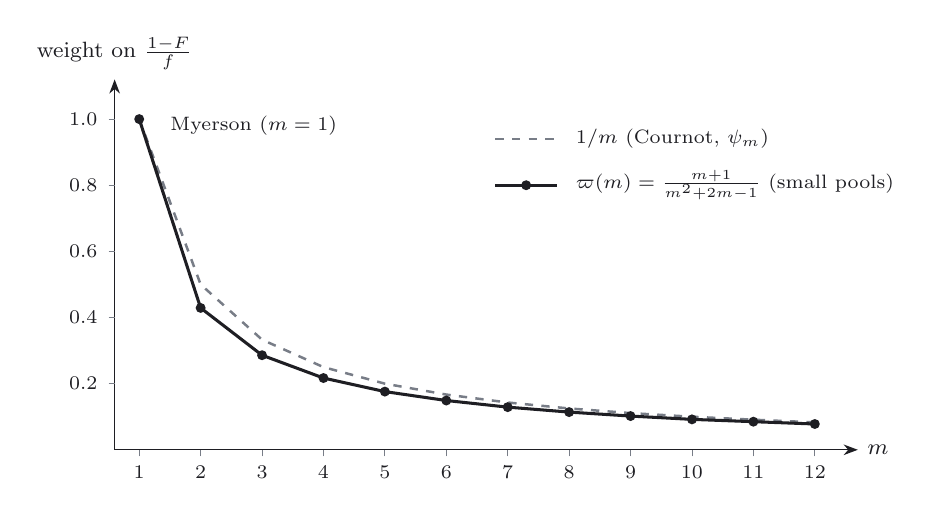
\begin{tikzpicture}[x=0.78cm,y=4.2cm]
  \draw[-{Stealth[length=1.8mm]},ink,line width=0.5pt] (0.6,0)--(12.7,0) node[right,font=\footnotesize]{$m$};
  \draw[-{Stealth[length=1.8mm]},ink,line width=0.5pt] (0.6,0)--(0.6,1.12) node[above,font=\footnotesize]{weight on $\frac{1-F}{f}$};
  \foreach \y in {0.2,0.4,0.6,0.8,1.0} {
    \draw[muted,line width=0.3pt] (0.50,\y)--(0.6,\y);
    \node[left,font=\scriptsize,text=ink] at (0.48,\y) {\y};
  }
  \foreach \x in {1,2,3,4,5,6,7,8,9,10,11,12} {
    \draw[muted,line width=0.3pt] (\x,-0.02)--(\x,0);
    \node[below,font=\scriptsize,text=ink] at (\x,-0.02) {\x};
  }
  % Cournot 1/m (dashed)
  \draw[muted,dashed,line width=0.9pt]
    (1,1.000)--(2,0.500)--(3,0.333)--(4,0.250)--(5,0.200)--(6,0.167)
    --(7,0.143)--(8,0.125)--(9,0.111)--(10,0.100)--(11,0.091)--(12,0.083);
  % Small-pool varpi(m) = (m+1)/(m^2+2m-1) (solid with circular dots)
  \draw[ink,line width=1.1pt]
    (1,1.000)--(2,0.429)--(3,0.286)--(4,0.217)--(5,0.176)--(6,0.149)
    --(7,0.129)--(8,0.114)--(9,0.102)--(10,0.092)--(11,0.085)--(12,0.078);
  \foreach \x/\y in {1/1.000,2/0.429,3/0.286,4/0.217,5/0.176,6/0.149,7/0.129,8/0.114,9/0.102,10/0.092,11/0.085,12/0.078}
    \fill[ink] (\x,\y) circle (1.8pt);
  \node[font=\scriptsize,text=ink,anchor=west] at (1.35,0.98) {Myerson ($m=1$)};
  % Legend
  \draw[muted,dashed,line width=0.9pt] (6.8,0.94)--(7.8,0.94);
  \node[font=\scriptsize,anchor=west,text=ink] at (7.95,0.94) {$1/m$ (Cournot, $\psi_m$)};
  \draw[ink,line width=1.1pt] (6.8,0.80)--(7.8,0.80);
  \fill[ink] (7.3,0.80) circle (1.8pt);
  \node[font=\scriptsize,anchor=west,text=ink] at (7.95,0.80) {$\varpi(m)=\frac{m+1}{m^2+2m-1}$ (small pools)};
\end{tikzpicture}
\caption{The weight on the inverse hazard rate from Myerson ($m=1$) to McAfee ($m\to\infty$). Dashed: Cournot's weight $1/m$, sufficient for every $n$ and sharp as $n\to\infty$. Solid: the small-pool weight $\varpi(m)$ of Proposition~\ref{prop:smallpool}.}
\label{fig:wm}
\end{figure}

\begin{proposition}[\textsc{Many Buyers}]\label{prop:manybuyers}
Against rivals at $\SPA(\rho)$, fix an interior band $[v_1,v_4]$ in $(\max\{\rho,a\},1)$ with quantities $\underline q<\bar q$, and let $D_n$ be the revenue change of the unique pool inducing that band at $n$ buyers.
\begin{enumerate}[(i)]
\item As $n\to\infty$,
\begin{equation}\label{eq:Jlim}
\lim_{n\to\infty}\frac{D_n}{(1-\underline q)^n} = \mathcal J(\underline q,\bar q) := \frac{\Pi(\bar q,\underline q)-\Pi(\underline q,\underline q)}{\bar q-\underline q} - \partial_t\Pi(\underline q,\underline q).
\end{equation}
\item $\mathcal J(\underline q,\bar q)\le 0$ for all $0<\underline q<\bar q<\frac{1-F(\max\{\rho,a\})}{m}$ if and only if $t\mapsto\Pi(t,q)$ lies below its tangent at $t=q$ on $[q,\frac{1-F(\max\{\rho,a\})}{m}]$. Under Assumption~\ref{a:two}, expanding for narrow bands ($d\downarrow 0$) gives $\mathcal J(q,q+d)=\frac{1}{2}\partial_{tt}\Pi(q,q)\,d+o(d)$, so the tangent condition requires $E\le 2m$ (and $\mathcal J(q,q+d)>0$ for small $d>0$ wherever $E(P(mq))>2m$).
\item For every $X>m+1$, there exists a covered-market distribution ($a>0$) satisfying Assumptions~\ref{a:one}--\ref{a:two} with $\psi_m(a)>0$ and $E\le X$ everywhere on $[a,1]$ that admits an interior band $[v_1,v_4]\subset(a,1)$ with $\mathcal J(\underline q,\bar q)>0$.
\end{enumerate}
\end{proposition}
\begin{proof}
For each $n\ge 2$, a unique pool induces $[v_1,v_4]$ by Lemma~\ref{lem:genband}(iii).

\emph{(i).} Write $A_4:=1-\underline q$ and $d:=\bar q-\underline q$. By Theorem~\ref{thm:cournot}, $D_n=n(n-1)(\mathcal I_1+\mathcal I_2)$ with $\mathcal I_1=\int_{\underline q}^{q^*}(1-q)^{n-2}[\Pi(\underline q,q)-\Pi(q,q)]\,dq$ and $\mathcal I_2=\int_{q^*}^{\bar q}(1-q)^{n-2}[\Pi(\bar q,q)-\Pi(q,q)]\,dq$. From \eqref{eq:qstar}, $(1-q^*)^{n-1}=\frac{A_4^n}{nd}(1+o(1))$, so $q^*\to\underline q$ and $n(q^*-\underline q)\to\infty$.
On $[\underline q,q^*]$, $P\in C^1$ gives $\Pi(\underline q,q)-\Pi(q,q)=-(\partial_t\Pi(\underline q,\underline q)+o(1))(q-\underline q)$. Since $\int_{\underline q}^1(q-\underline q)(1-q)^{n-2}\,dq=\frac{A_4^n}{n(n-1)}$ and the tail above $q^*$ is $o(A_4^n/n^2)$, we have $n(n-1)\mathcal I_1=-\partial_t\Pi(\underline q,\underline q)A_4^n+o(A_4^n)$.
On $[q^*,\bar q]$, $(1-q)^{n-2}$ concentrates at $q^*\to\underline q$ with total mass $\frac{(1-q^*)^{n-1}-(1-\bar q)^{n-1}}{n-1}=\frac{A_4^n}{n(n-1)d}(1+o(1))$, so $n(n-1)\mathcal I_2=\frac{\Pi(\bar q,\underline q)-\Pi(\underline q,\underline q)}{d}A_4^n+o(A_4^n)$. Adding gives \eqref{eq:Jlim}.

\emph{(ii).} The tangent equivalence is immediate from \eqref{eq:Jlim}. Under Assumption~\ref{a:two},
\[
\mathcal J(q,q+d) = \frac{1}{2}\,\partial_{tt}\Pi(q,q)\,d + o(d) = \frac{1}{2}\,P'(mq)\Bigl(2-\frac{E(P(mq))}{m}\Bigr)\,d + o(d).
\]

\emph{(iii).} Fix $X>m+1$. Consider $\phi_X(u):=u(u+m-1)^{1-X}-m^{1-X}u+(X-1)m^{-X}(u-1)$ for $u>1$. Since $\phi_X(u)/u\to m^{-X}(X-1-m)>0$ as $u\to\infty$, pick $u>1$ large enough that $\phi_X(u)>0$, and choose $z_0>0$ small enough that $z_1:=\frac{u+m-1}{m}z_0<1$ and $u z_0<1$. Let $\tilde E:[0,1]\to[0,X]$ be continuous with $\tilde E(z)=X$ on $[z_0,z_1]$ and $\tilde E(z)=0$ on $[0,z_0/2]$. For $\kappa>0$, define
\[
P'(z) := -\kappa\exp\Bigl(-\int_{z_0}^z \frac{\tilde E(s)}{s}\,ds\Bigr), \qquad P(z) := 1 + \int_0^z P'(s)\,ds
\]
on $[0,1]$. Then $P\in C^2([0,1])$ with $P'<0$ everywhere and $P(0)=1$, so $F(v):=1-P^{-1}(v)$ on $[a,1]$ (where $a:=P(1)=1-\kappa C_0$ for $C_0:=\int_0^1 |P'(s)/\kappa|\,ds>0$) satisfies Assumptions~\ref{a:one}--\ref{a:two}. Moreover, $E(P(z))=-\frac{zP''(z)}{P'(z)}=\tilde E(z)\in[0,X]$ everywhere on $[0,1]$. Choosing $\kappa>0$ small enough yields $a=1-\kappa C_0>0$ and $\psi_m(a)=a+\frac{1}{m}P'(1)>0$. On $[z_0,z_1]$, $P'(z)=-\kappa(z/z_0)^{-X}$, so $P(z)=c_1+\frac{\kappa z_0^X}{X-1}z^{1-X}$ for a constant $c_1$. Setting $\underline q:=z_0/m$ and $\bar q:=u\underline q$ (so $m\underline q=z_0$ and $\bar q+(m-1)\underline q=z_1<1$, and $m\bar q=uz_0<1$), direct evaluation gives
\[
\Pi(\bar q,\underline q)-\Pi(\underline q,\underline q)-\partial_t\Pi(\underline q,\underline q)(\bar q-\underline q) = \frac{\kappa z_0^X}{X-1}\,\underline q^{2-X}\,\phi_X(u) > 0,
\]
so the interior band $[P(m\bar q),P(m\underline q)]\subset(a,1)$ satisfies $\mathcal J(\underline q,\bar q)>0$.
\end{proof}

Together, Theorem~\ref{thm:cournot}(ii) and Propositions~\ref{prop:smallpool}--\ref{prop:manybuyers} establish Theorem~\ref{thm:sharp}.

%%%%%%%%%%%%%%%%%%%%%%%%%%%%%%
% Bibliography
%%%%%%%%%%%%%%%%%%%%%%%%%%%%%%
\begin{thebibliography}{99}

\bibitem[Albrecht et~al.(2014)]{albrecht2014} Albrecht, J., P.~A. Gautier, and S.~Vroman (2014): ``Efficient Entry in Competing Auctions,'' \emph{American Economic Review}, 104(10), 3288--3296.

\bibitem[Armstrong and Vickers(2001)]{armstrong2001} Armstrong, M., and J.~Vickers (2001): ``Competitive Price Discrimination,'' \emph{RAND Journal of Economics}, 32(4), 579--605.

\bibitem[Azevedo and Budish(2019)]{azevedo2019} Azevedo, E.~M., and E.~Budish (2019): ``Strategy-proofness in the Large,'' \emph{Review of Economic Studies}, 86(1), 81--116.

\bibitem[Biais et~al.(2000)]{biais2000} Biais, B., D.~Martimort, and J.-C. Rochet (2000): ``Competing Mechanisms in a Common Value Environment,'' \emph{Econometrica}, 68(4), 799--837.

\bibitem[Border(1991)]{border1} Border, K.~C. (1991): ``Implementation of Reduced Form Auctions: A Geometric Approach,'' \emph{Econometrica}, 59(4), 1175--1187.

\bibitem[Bresnahan(1989)]{bresnahan1989} Bresnahan, T.~F. (1989): ``Empirical Studies of Industries with Market Power,'' in \emph{Handbook of Industrial Organization}, vol.~2, ed. by R.~Schmalensee and R.~D. Willig. North-Holland, Amsterdam, 1011--1057.

\bibitem[Bulow and Roberts(1989)]{bulow1989} Bulow, J., and J.~Roberts (1989): ``The Simple Economics of Optimal Auctions,'' \emph{Journal of Political Economy}, 97(5), 1060--1090.

\bibitem[Burdett et~al.(2001)]{burdett2001pricing} Burdett, K., S.~Shi, and R.~Wright (2001): ``Pricing and Matching with Frictions,'' \emph{Journal of Political Economy}, 109(5), 1060--1085.

\bibitem[Burguet and S{\'a}kovics(1999)]{burguet} Burguet, R., and J.~S{\'a}kovics (1999): ``Imperfect Competition in Auction Designs,'' \emph{International Economic Review}, 40(1), 231--247.

\bibitem[Chade and Swinkels(2021)]{chade2021} Chade, H., and J.~Swinkels (2021): ``Screening in Vertical Oligopolies,'' \emph{Econometrica}, 89(3), 1265--1311.

\bibitem[Che et~al.(2013)]{che2013} Che, Y.-K., J.~Kim, and K.~Mierendorff (2013): ``Generalized Reduced-Form Auctions: A Network-Flow Approach,'' \emph{Econometrica}, 81(6), 2487--2520.

\bibitem[Davidson and Deneckere(1986)]{davidson} Davidson, C., and R.~Deneckere (1986): ``Long-Run Competition in Capacity, Short-Run Competition in Price, and the Cournot Model,'' \emph{RAND Journal of Economics}, 17(3), 404--415.

\bibitem[Dworczak et~al.(2021)]{dworczak2021} Dworczak, P., S.~D. Kominers, and M.~Akbarpour (2021): ``Redistribution through Markets,'' \emph{Econometrica}, 89(4), 1665--1698.

\bibitem[Eeckhout and Kircher(2010)]{eeckhout2010sorting} Eeckhout, J., and P.~Kircher (2010): ``Sorting versus Screening: Search Frictions and Competing Mechanisms,'' \emph{Journal of Economic Theory}, 145(4), 1354--1385.

\bibitem[Einav et~al.(2018)]{einav2018} Einav, L., C.~Farronato, J.~Levin, and N.~Sundaresan (2018): ``Auctions versus Posted Prices in Online Markets,'' \emph{Journal of Political Economy}, 126(1), 178--215.

\bibitem[Epstein and Peters(1999)]{epstein1999} Epstein, L.~G., and M.~Peters (1999): ``A Revelation Principle for Competing Mechanisms,'' \emph{Journal of Economic Theory}, 88(1), 119--160.

\bibitem[Glicksberg(1952)]{glicksberg1952} Glicksberg, I.~L. (1952): ``A Further Generalization of the Kakutani Fixed Point Theorem, with Application to Nash Equilibrium Points,'' \emph{Proceedings of the American Mathematical Society}, 3(1), 170--174.

\bibitem[Hart and Reny(2015)]{hartreny2015} Hart, S., and P.~J. Reny (2015): ``Implementation of Reduced Form Mechanisms: A Simple Approach and a New Characterization,'' \emph{Economic Theory Bulletin}, 3(1), 1--8.

\bibitem[He(2026)]{he2026} He, N. (2026): ``Buyer Sorting and Reserve Differentiation among Competing Sellers,'' working paper, University of Southern California.

\bibitem[Hernando-Veciana(2005)]{hernando2005} Hernando-Veciana, A. (2005): ``Competition among Auctioneers in Large Markets,'' \emph{Journal of Economic Theory}, 121(1), 107--127.

\bibitem[Jullien(2000)]{jullien} Jullien, B. (2000): ``Participation Constraints in Adverse Selection Models,'' \emph{Journal of Economic Theory}, 93(1), 1--47.

\bibitem[Kim and Kircher(2015)]{kim2015} Kim, K., and P.~Kircher (2015): ``Efficient Competition through Cheap Talk: The Case of Competing Auctions,'' \emph{Econometrica}, 83(5), 1849--1875.

\bibitem[Kleiner et~al.(2021)]{kleiner2021} Kleiner, A., B.~Moldovanu, and P.~Strack (2021): ``Extreme Points and Majorization: Economic Applications,'' \emph{Econometrica}, 89(4), 1557--1593.

\bibitem[Kreps and Scheinkman(1983)]{kreps} Kreps, D.~M., and J.~A. Scheinkman (1983): ``Quantity Precommitment and Bertrand Competition Yield Cournot Outcomes,'' \emph{Bell Journal of Economics}, 14(2), 326--337.

\bibitem[Lester et~al.(2017)]{lester2017} Lester, B., L.~Visschers, and R.~Wolthoff (2017): ``Competing with Asking Prices,'' \emph{Theoretical Economics}, 12(2), 731--770.

\bibitem[Ma and Riquelme(2026)]{ma2026} Ma, Z., and N.~Riquelme (2026): ``Competitive Limit of Competing Auctions,'' \emph{Games and Economic Behavior}, 158, 367--382.

\bibitem[Manelli and Vincent(2010)]{manelli2010} Manelli, A.~M., and D.~R. Vincent (2010): ``Bayesian and Dominant-Strategy Implementation in the Independent Private-Values Model,'' \emph{Econometrica}, 78(6), 1905--1938.

\bibitem[McAfee(1993)]{mcafee} McAfee, R.~P. (1993): ``Mechanism Design by Competing Sellers,'' \emph{Econometrica}, 61(6), 1281--1312.

\bibitem[Moldovanu et~al.(2008)]{moldovanu} Moldovanu, B., A.~Sela, and X.~Shi (2008): ``Competing Auctions with Endogenous Quantities,'' \emph{Journal of Economic Theory}, 141(1), 1--27.

\bibitem[Monderer and Shapley(1996)]{monderer1996} Monderer, D., and L.~S. Shapley (1996): ``Potential Games,'' \emph{Games and Economic Behavior}, 14(1), 124--143.

\bibitem[Myerson(1981)]{myerson} Myerson, R.~B. (1981): ``Optimal Auction Design,'' \emph{Mathematics of Operations Research}, 6(1), 58--73.

\bibitem[Peters(1997)]{peters1997} Peters, M. (1997): ``A Competitive Distribution of Auctions,'' \emph{Review of Economic Studies}, 64(1), 97--123.

\bibitem[Peters(2001)]{peters2001common} Peters, M. (2001): ``Common Agency and the Revelation Principle,'' \emph{Econometrica}, 69(5), 1349--1372.

\bibitem[Peters and Severinov(1997)]{peters} Peters, M., and S.~Severinov (1997): ``Competition among Sellers Who Offer Auctions Instead of Prices,'' \emph{Journal of Economic Theory}, 75(1), 141--179.

\bibitem[Rochet and Stole(2002)]{rochet} Rochet, J.-C., and L.~A. Stole (2002): ``Nonlinear Pricing with Random Participation,'' \emph{Review of Economic Studies}, 69(1), 277--311.

\bibitem[Stole(2007)]{stole2007} Stole, L.~A. (2007): ``Price Discrimination and Competition,'' in \emph{Handbook of Industrial Organization}, vol.~3, ed. by M.~Armstrong and R.~Porter. Elsevier, Amsterdam, 2221--2299.

\bibitem[Toikka(2011)]{toikka2011} Toikka, J. (2011): ``Ironing without Control,'' \emph{Journal of Economic Theory}, 146(6), 2510--2526.

\bibitem[Vetta(2002)]{vetta2002} Vetta, A. (2002): ``Nash Equilibria in Competitive Societies, with Applications to Facility Location, Traffic Routing and Auctions,'' in \emph{Proceedings of the 43rd IEEE Symposium on Foundations of Computer Science}, IEEE Computer Society, 416--425.

\bibitem[Vir{\'a}g(2007)]{virag} Vir{\'a}g, G. (2007): ``Buyer Heterogeneity and Competing Mechanisms,'' working paper, University of Rochester.

\bibitem[Vir{\'a}g(2010)]{virag2010competing} Vir{\'a}g, G. (2010): ``Competing Auctions: Finite Markets and Convergence,'' \emph{Theoretical Economics}, 5(2), 241--274.

\bibitem[Weyl and Fabinger(2013)]{weyl2013} Weyl, E.~G., and M.~Fabinger (2013): ``Pass-Through as an Economic Tool: Principles of Incidence under Imperfect Competition,'' \emph{Journal of Political Economy}, 121(3), 528--583.

\bibitem[Wright et~al.(2021)]{wright2021} Wright, R., P.~Kircher, B.~Julien, and V.~Guerrieri (2021): ``Directed Search and Competitive Search Equilibrium: A Guided Tour,'' \emph{Journal of Economic Literature}, 59(1), 90--148.

\bibitem[Yang and Ye(2008)]{yang2008} Yang, H., and L.~Ye (2008): ``Nonlinear Pricing, Market Coverage, and Competition,'' \emph{Theoretical Economics}, 3(1), 123--153.

\end{thebibliography}

\end{document}
